\documentclass[11pt,letterpaper]{article}
\input{headings}
\newcommand \recipeName {Daniel's Pasta}
\newcommand \fileName {DanielsPasta}
\chead{\recipeName}

\begin{document}
\input{title}

\begin{flushright}
{\bf From {\it } by }
\end{flushright}
 
\begin{description}

\item[Ingredients:]\ \\
	\begin{itemize}
	\item 2 Tablespoons of olive oil
	\item 200 grams of dried store-bought pasta such as macaroni, penne, gemelli
	\item 250 grams of \href{DanielsMeatSauce.html}{Daniel's Meat Sauce}
	\item 2 cups (16 oz) of water
	\item 3 Tablespoons of freshly grated parmesan cheese 
	\item Freshly grated black pepper
	\end{itemize}

\item[Procedure:]\ \\
	\begin{enumerate}
	\item {\bf Brown and boil the pasta}
	\begin{itemize}
	\item Put the olive oil in a large frying pan (non sticking is better), put over moderate high heat.
        \item Dump the pasta in the oil
	\item Stir fry constantly with a wooden spoon or by shaking the pan until the pasta is lightly browned all over.
	\item Add the water to the browned pasta, adjust the heat to medium, cover the pan.
	
	\item Check after 7 minutes:
		\begin{itemize} 
			\item If it looks like the pasta is cooking fast and there is still lots of liquid, let it cook uncovered in higher heat for a minute or two to evaporate the water faster. 
			\item If it looks like it is getting dry and the past is still not quite al-dente, add another 1/2 cup or so of water and cook it covered a little longer.
		\end{itemize}
	\item Cook until the liquid has evaporated and the pasta is very al-dente (total cooking time should be 8 to 10 minutes). 
	\end{itemize}
	\item {\bf Warm up the sauce}
	\begin{itemize}
	\item Warm up the sauce in the microwave. Easier if you have portioned the sauce in microwave-safe small dishes and froze it. You can thaw the sauce directly in the microwave. You want to have the sauce very warm
	\item Dump all the sauce at once over the al-dente pasta and adjust the heat to moderate high.
	\item Cook the pasta with the sauce stirring constantly with a wooden spoon for about 3 minutes.
	\item Turn off the heat and season with freshly ground pepper.
	\item Put in a plate and sprinkle with the parmesan cheese.
	\item At this point the pasta will be quite dry with the sauce clinging to it. This is exactly how Daniel likes it.
	\item However most people like their pasta to have some sauce. In this case simply add about 1/4 cup of water to the pan at the end and scrape all the edges of the pan to make a sauce. 
	\end{itemize}
	\end{enumerate}
\end{description}

\begin{table}
\begin{tabular}{cccc}
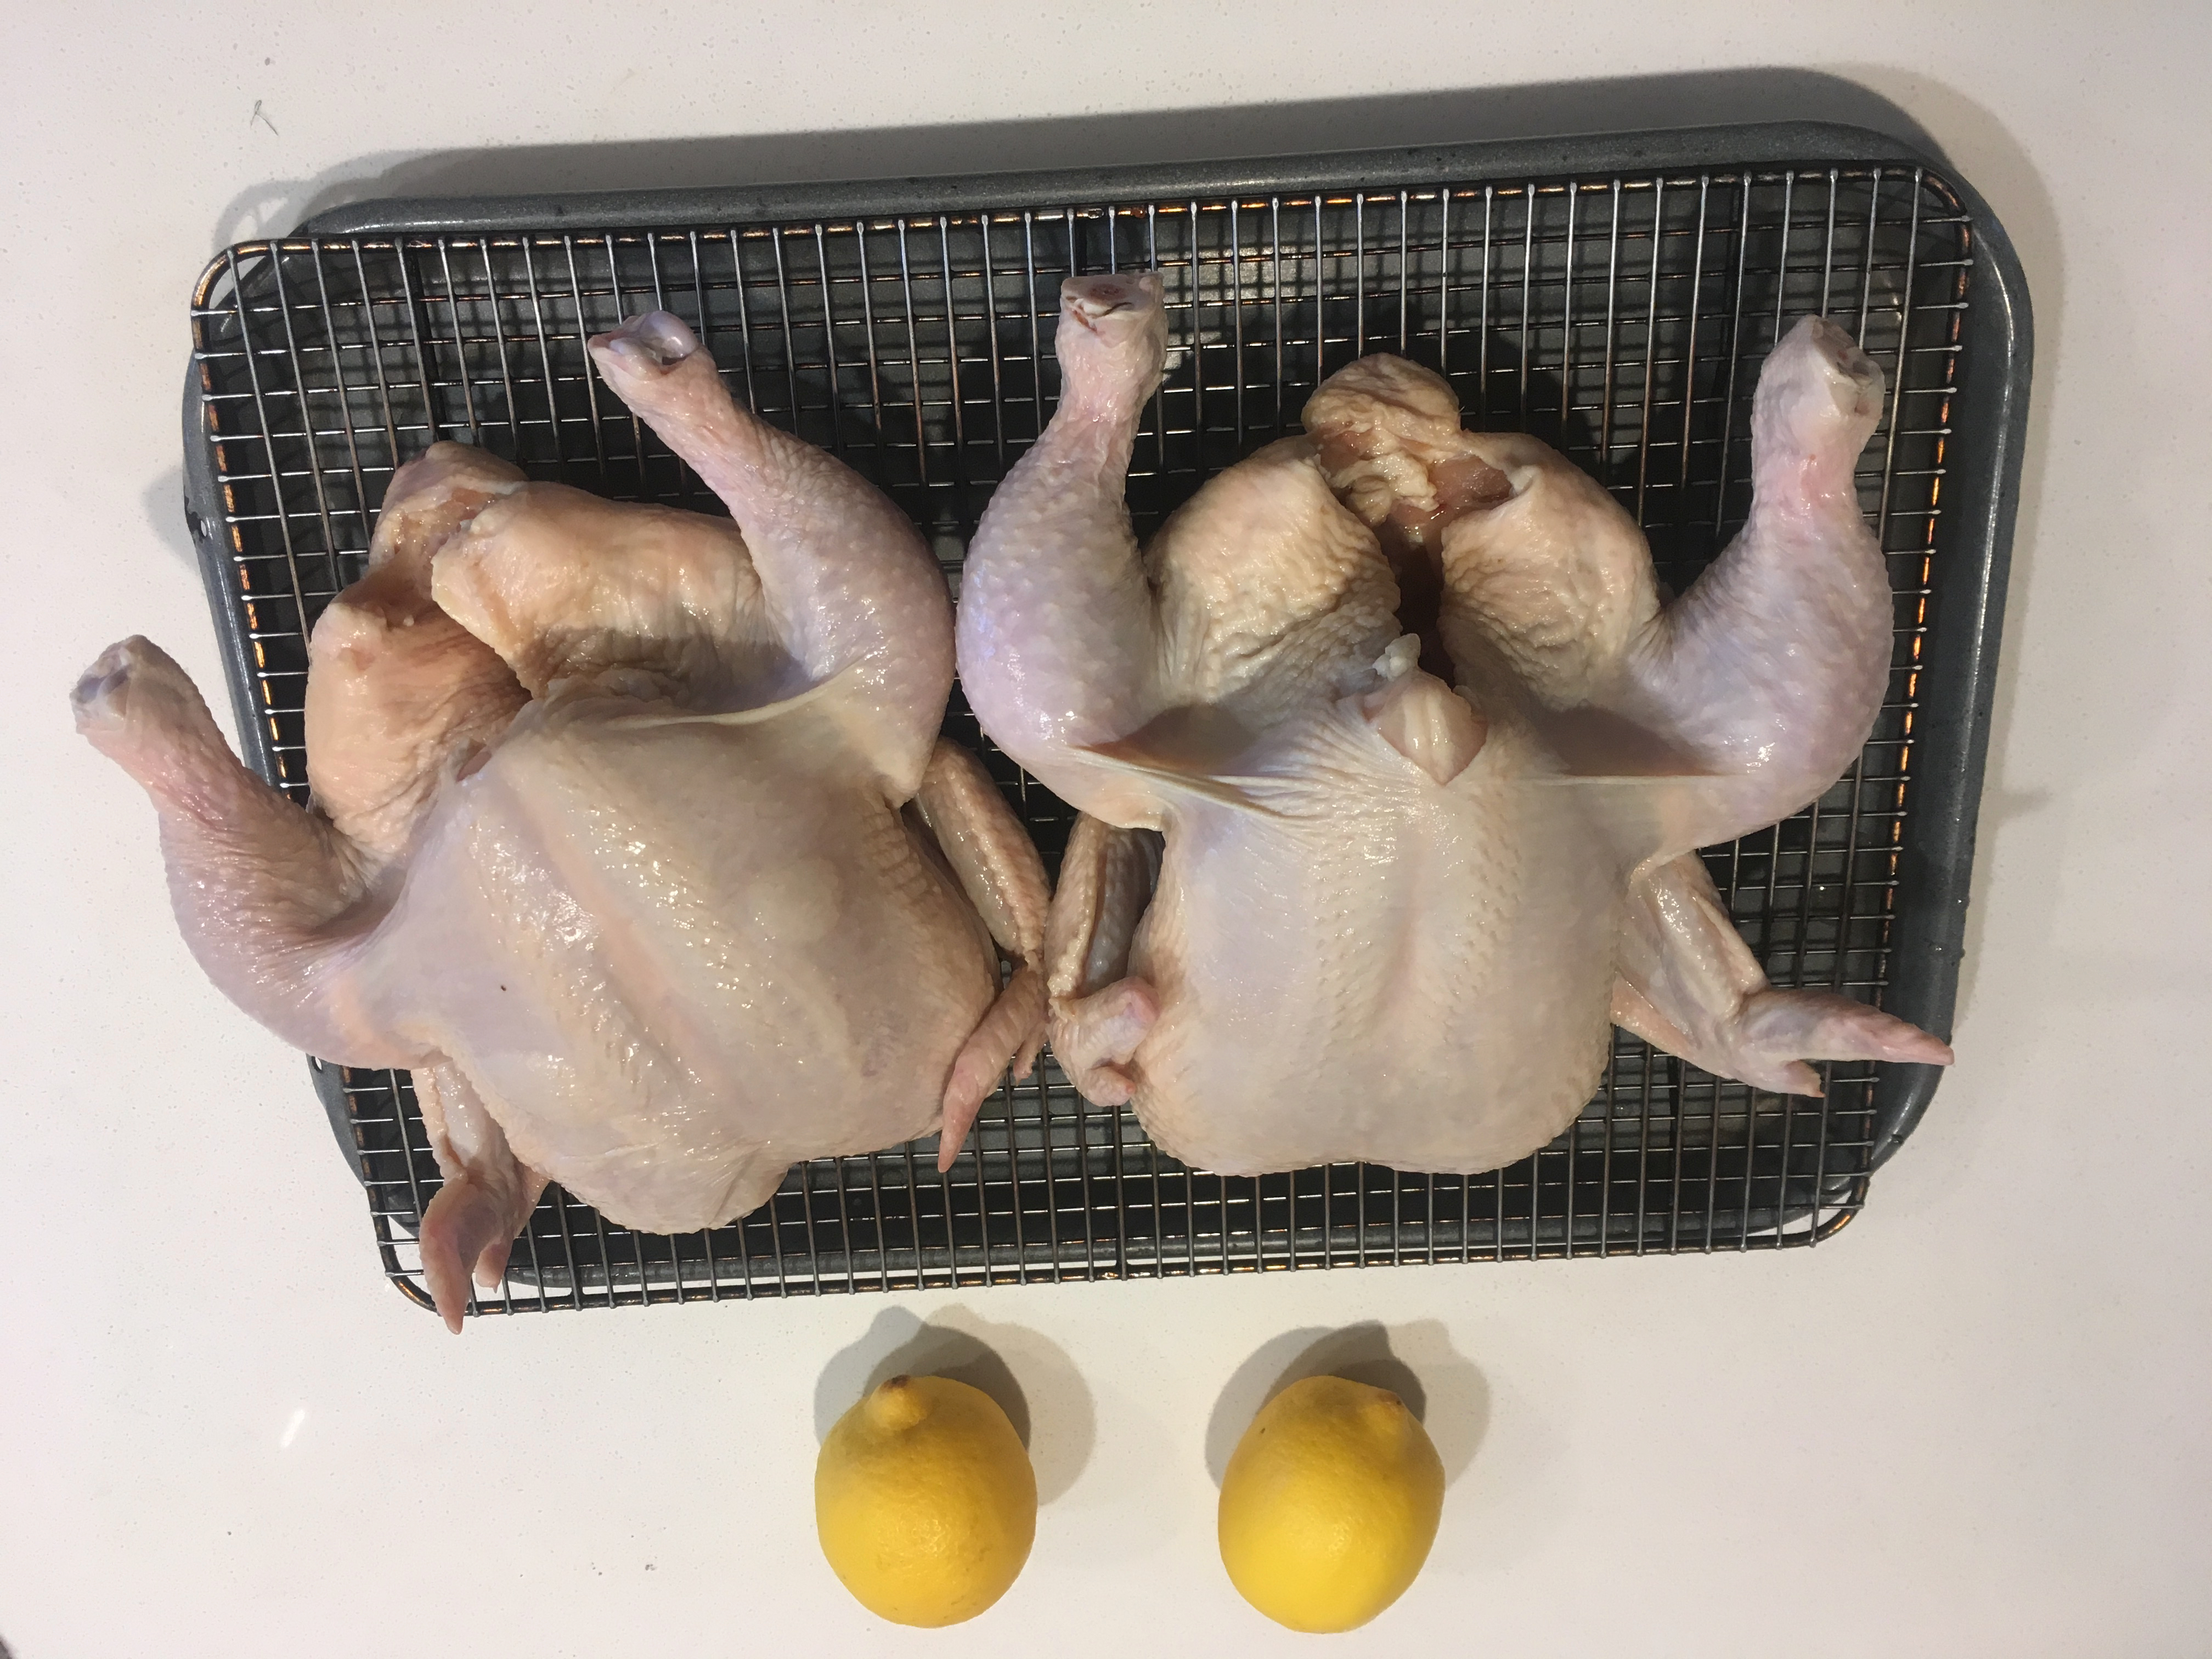
\includegraphics[width=0.25\textwidth]{\imageDir/\fileName/IMG_3197.jpg} &
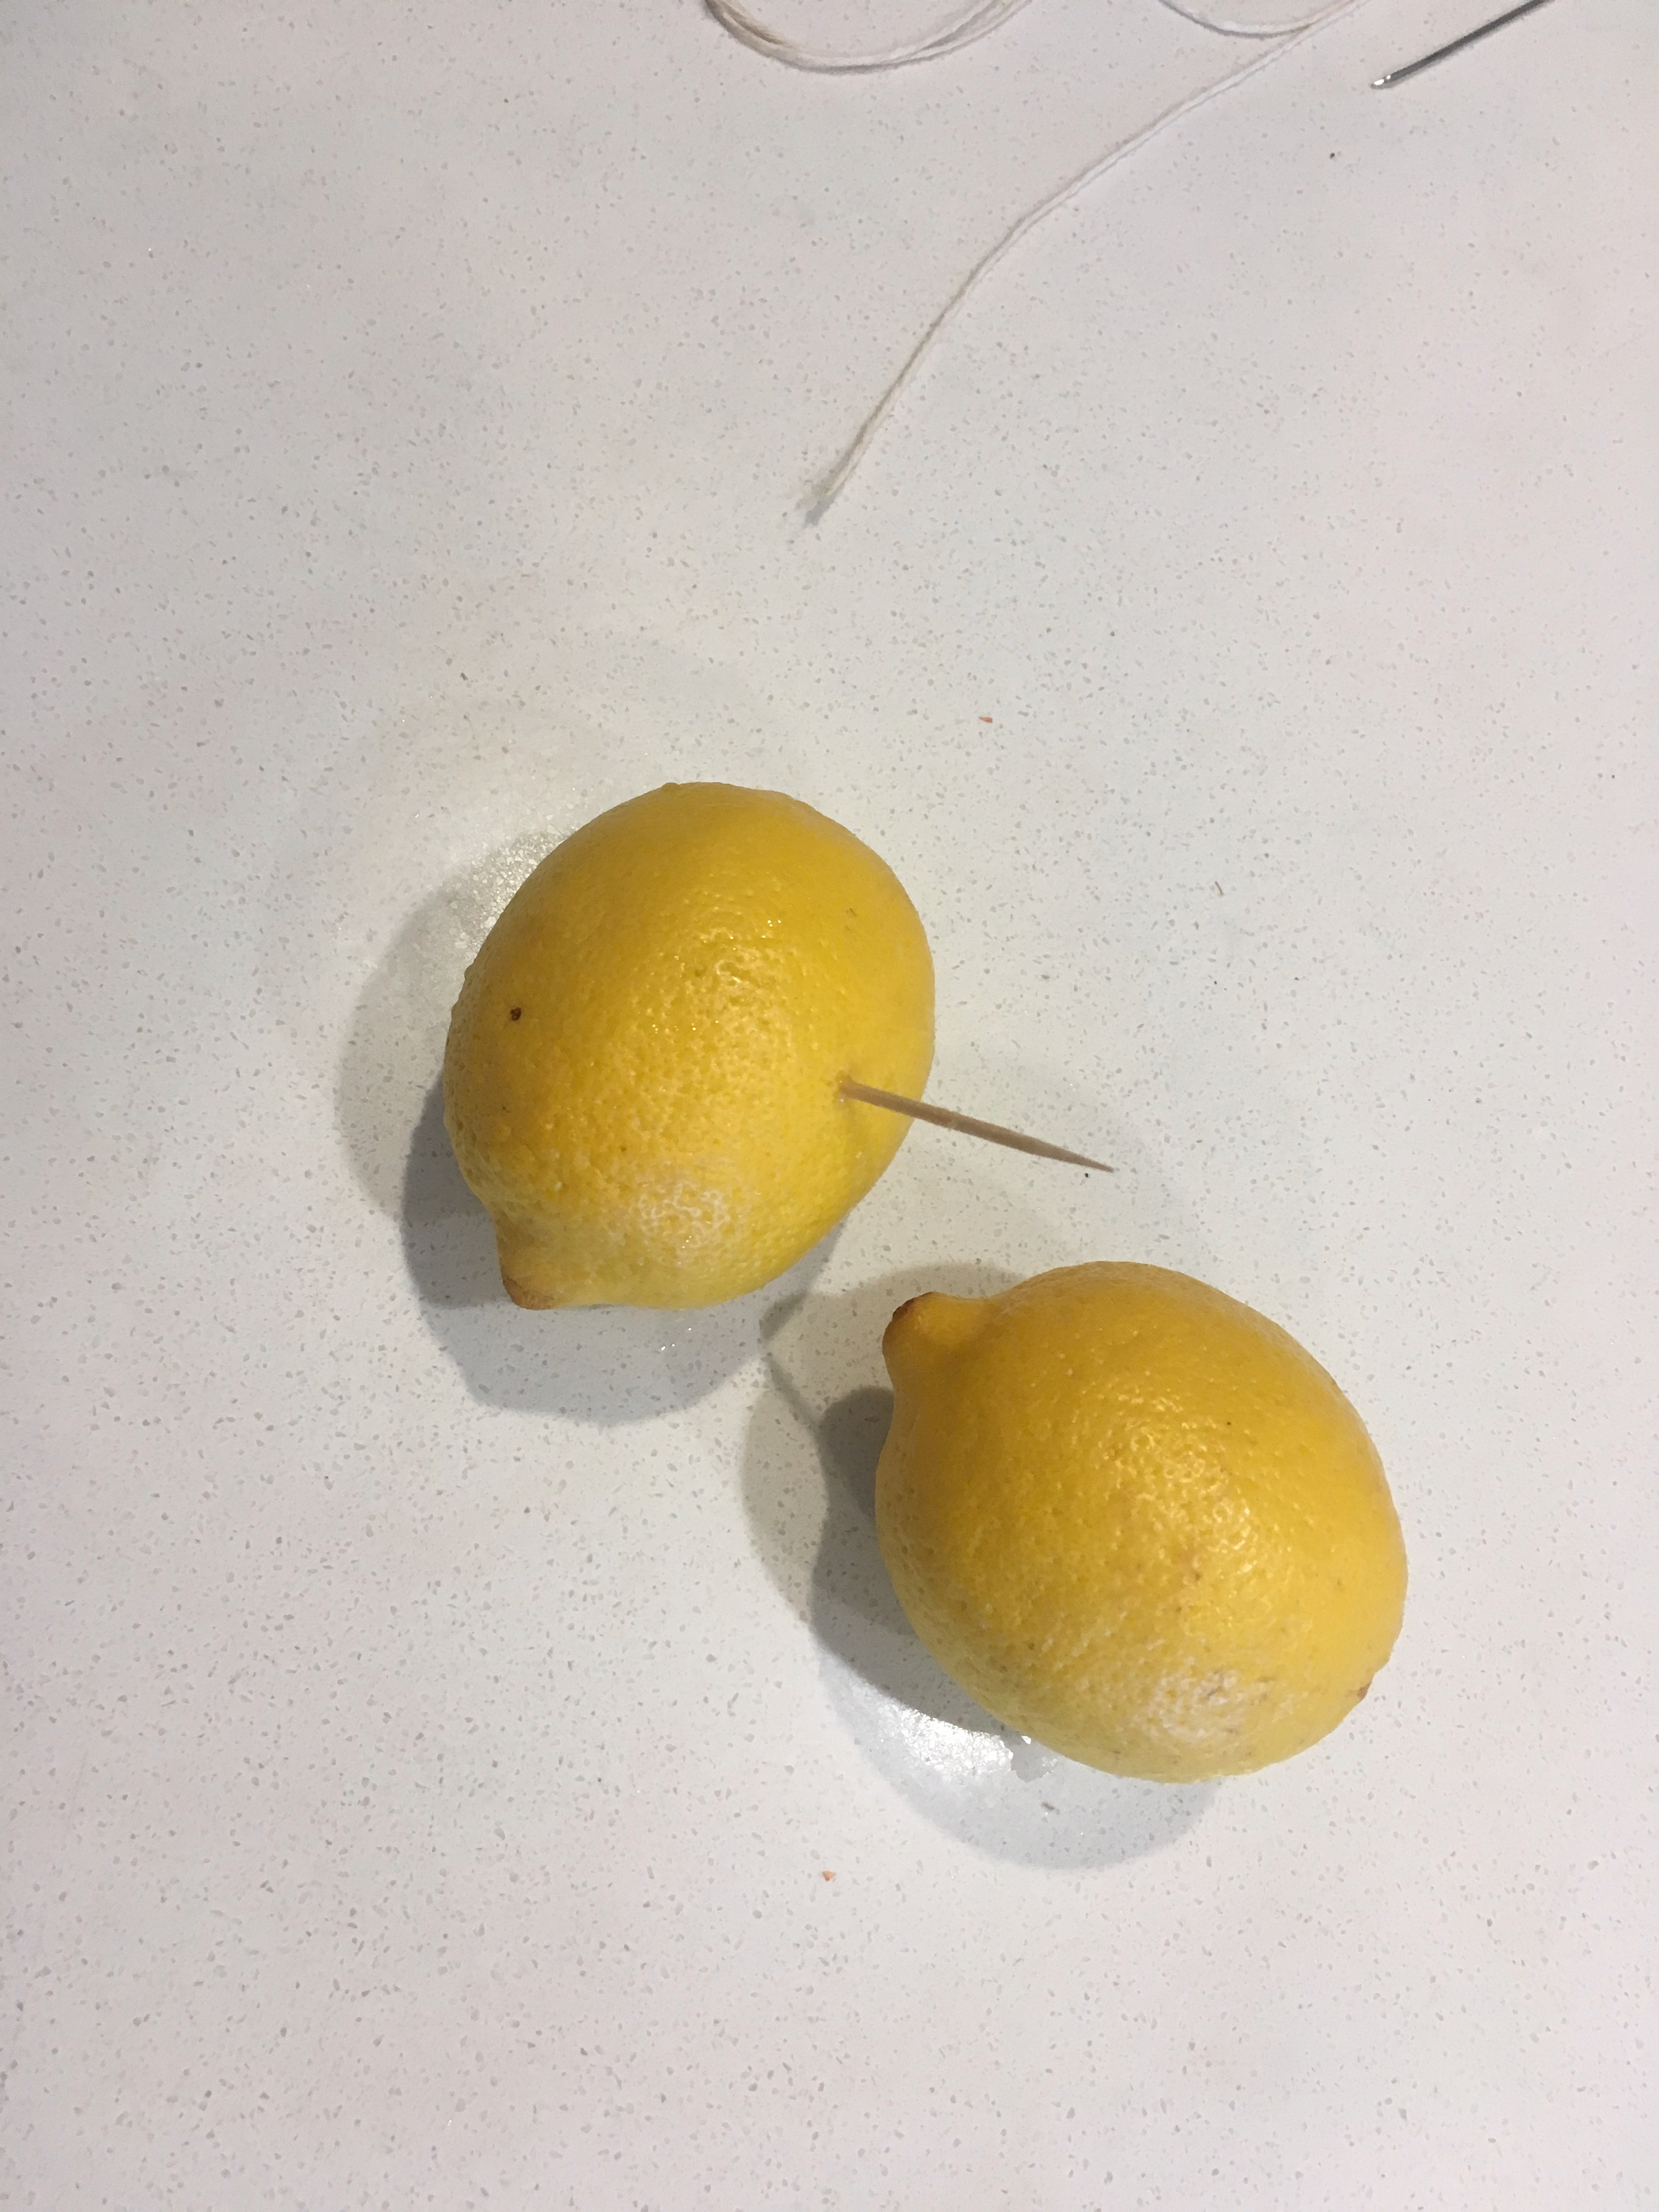
\includegraphics[width=0.25\textwidth]{\imageDir/\fileName/IMG_3212.jpg} &
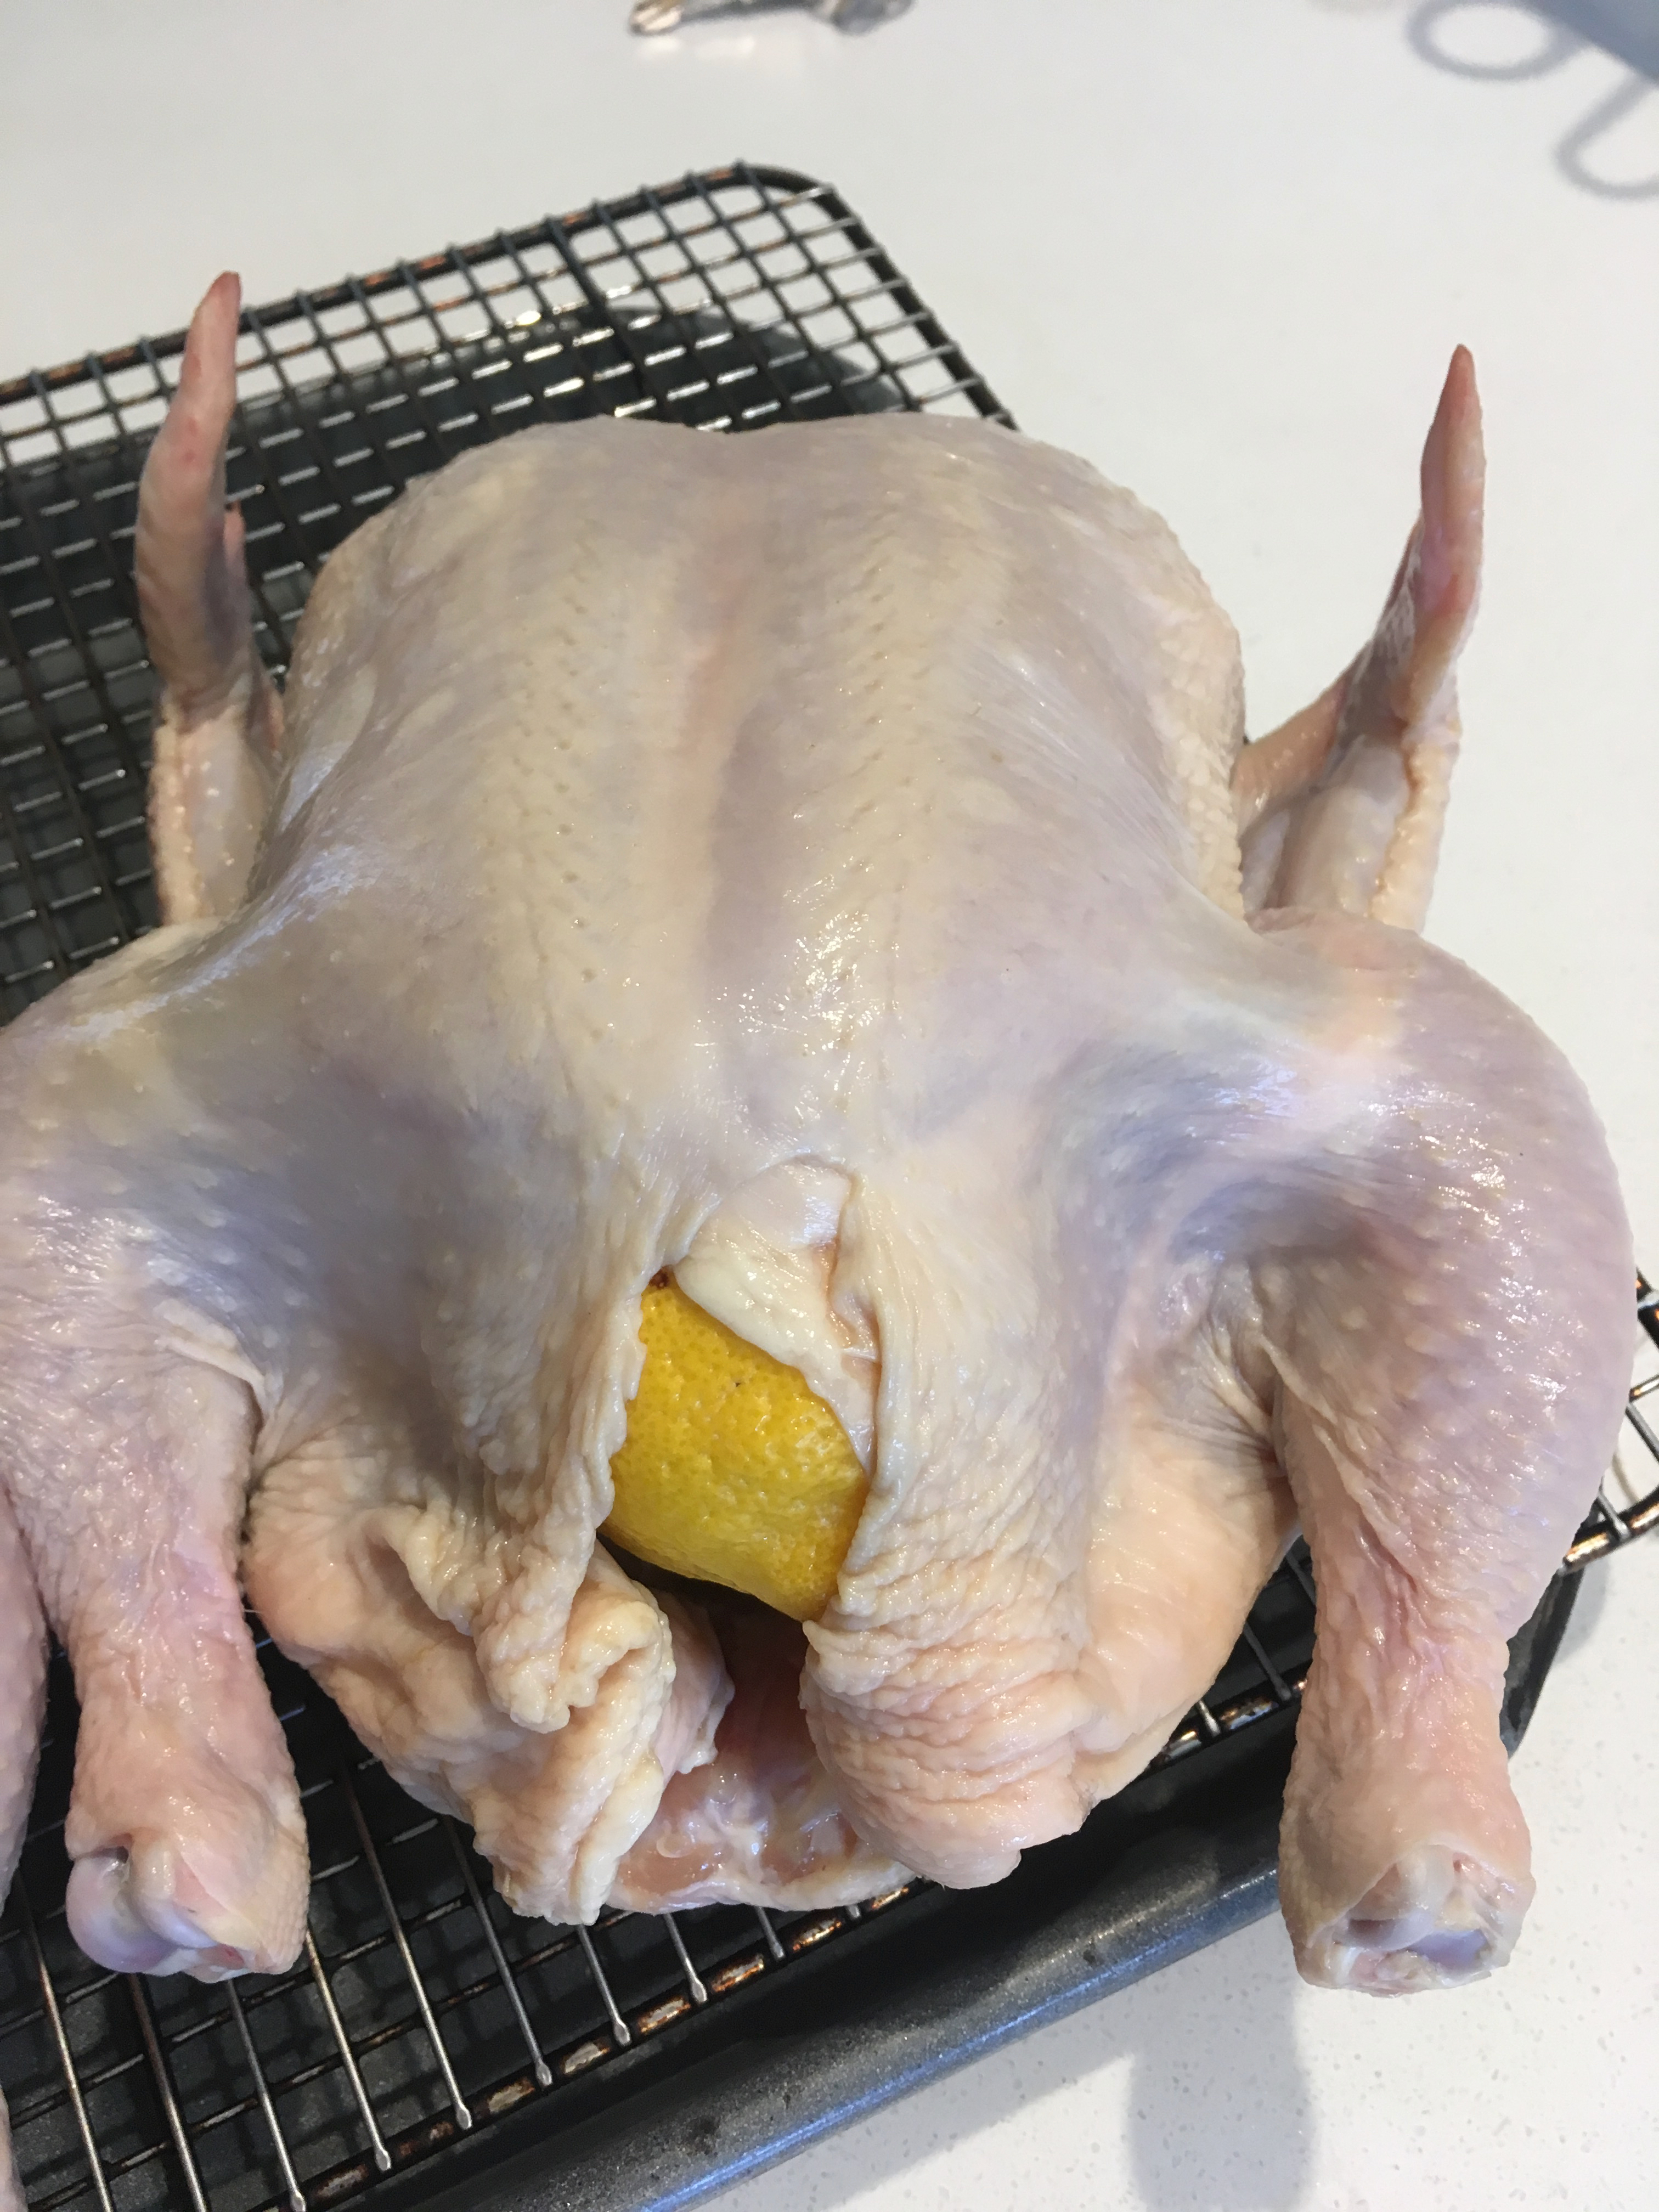
\includegraphics[width=0.25\textwidth]{\imageDir/\fileName/IMG_3213.jpg} \\
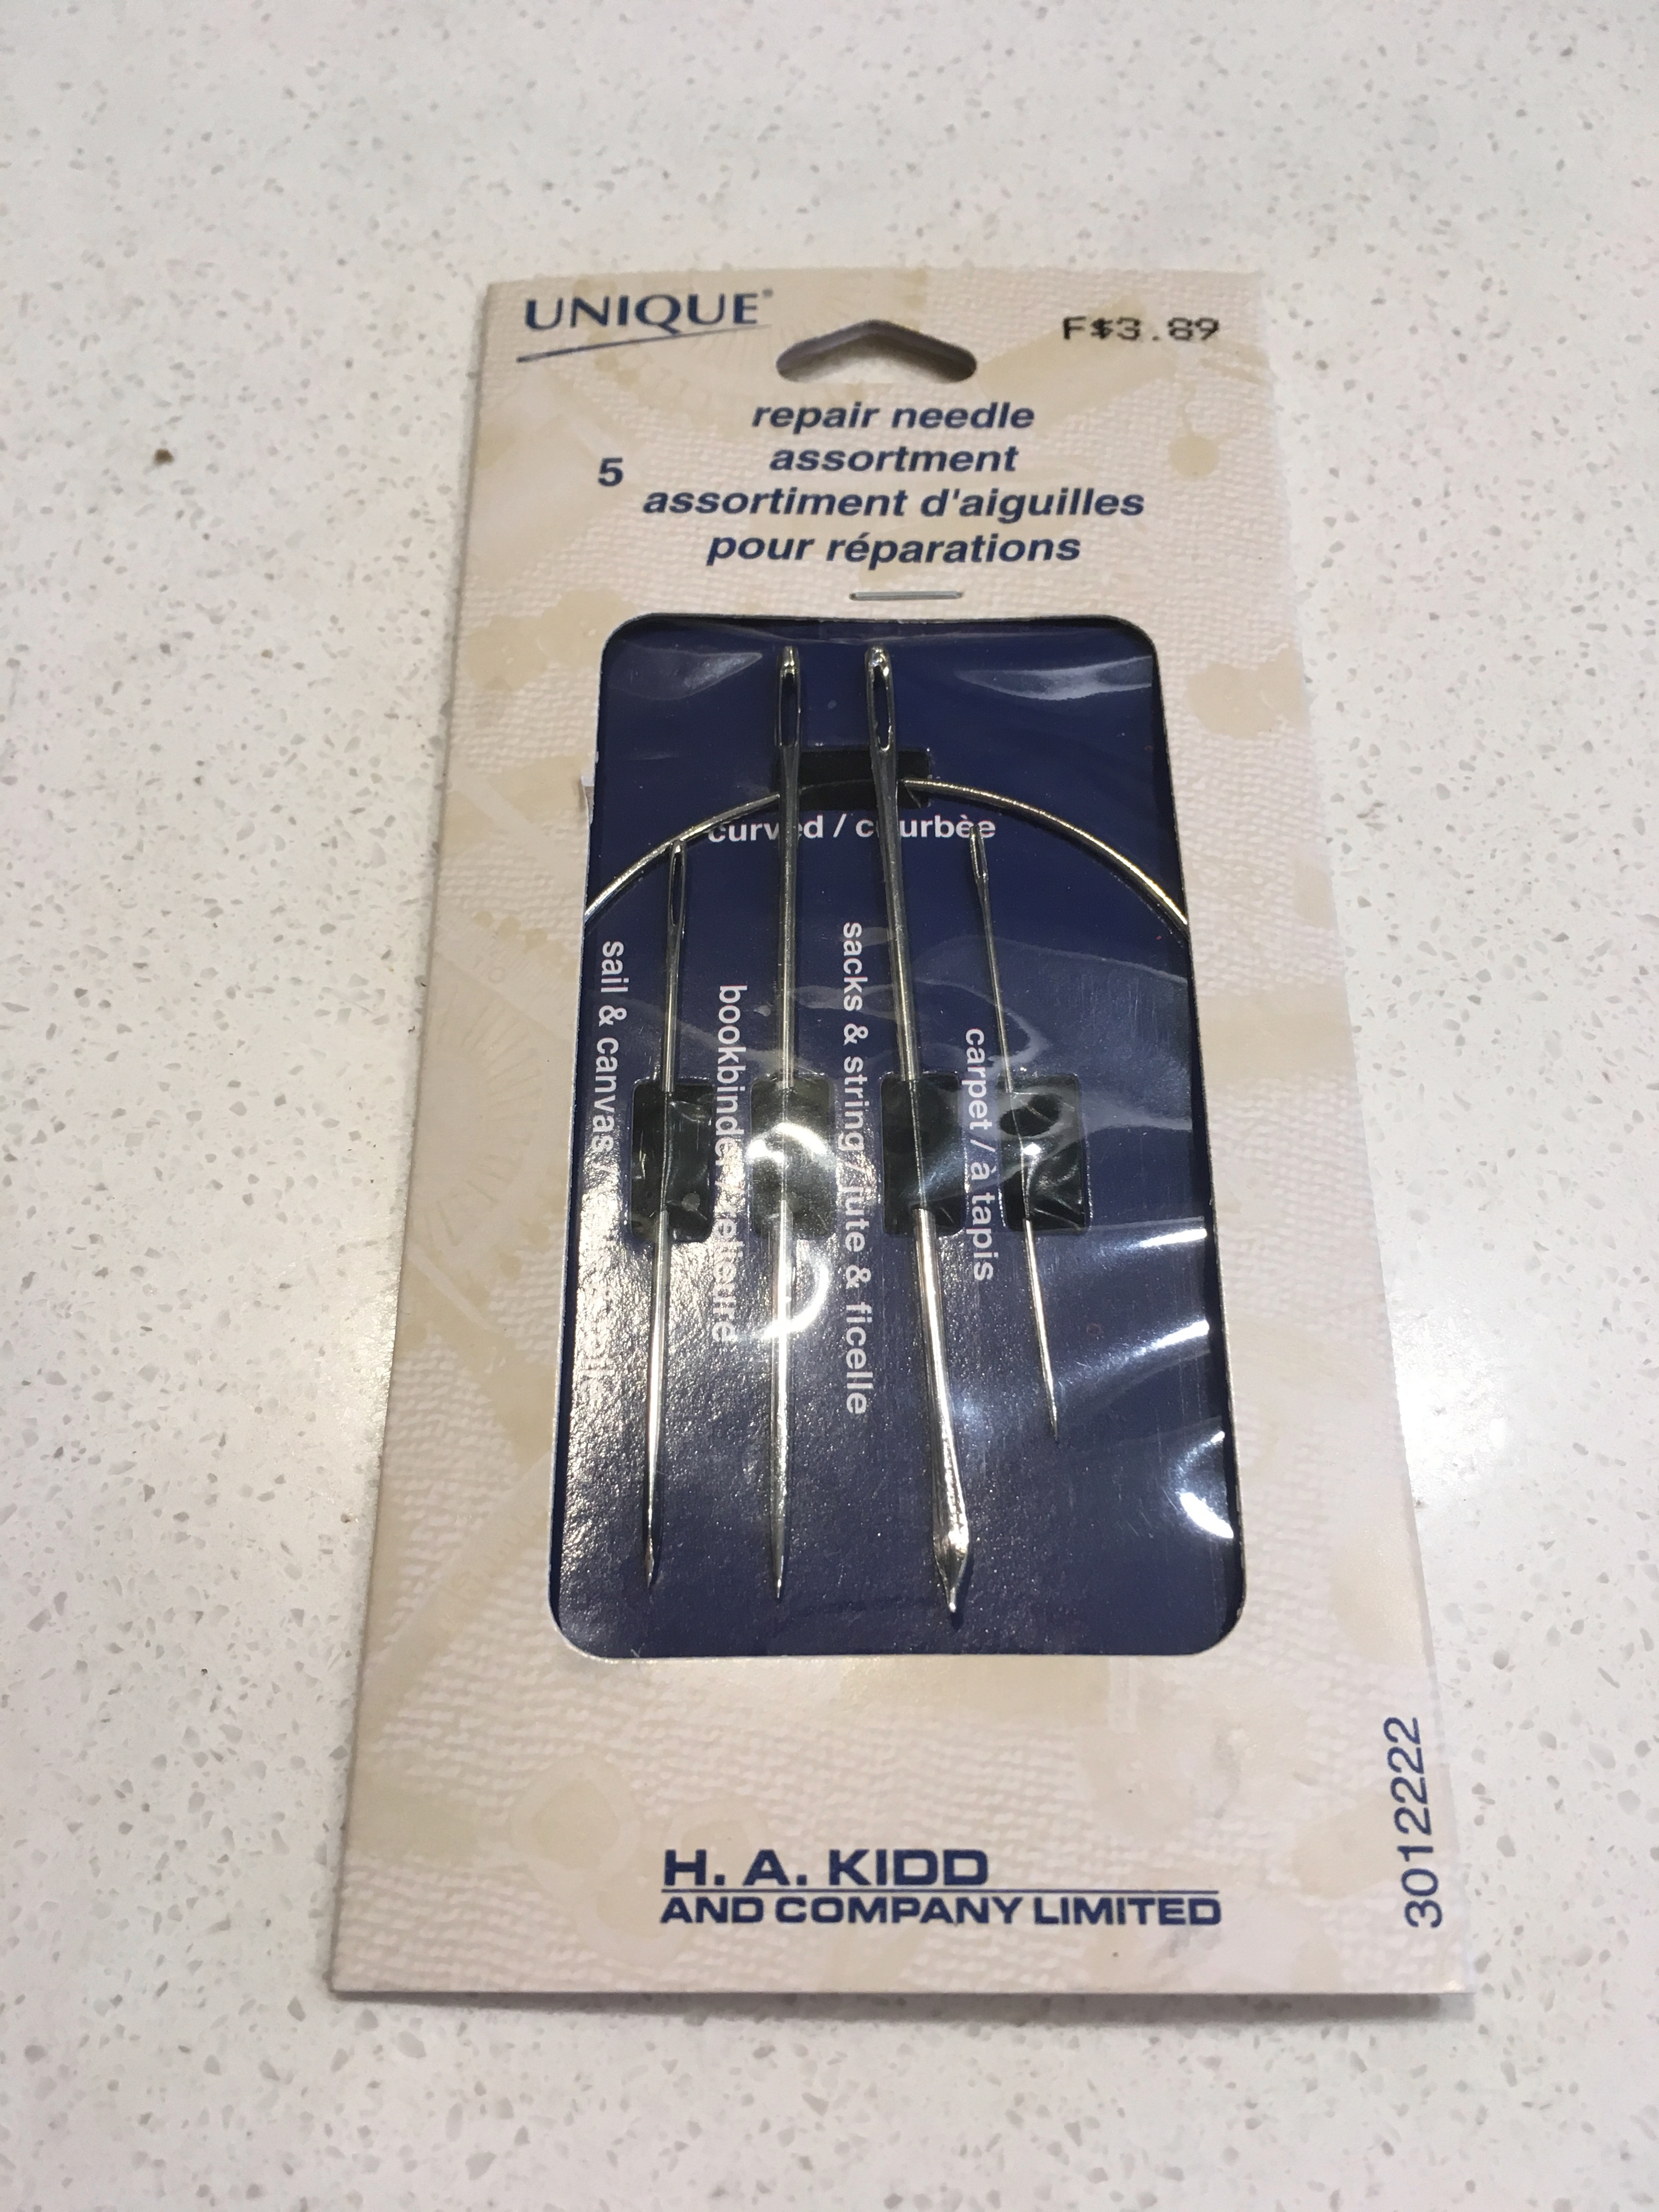
\includegraphics[width=0.25\textwidth]{\imageDir/\fileName/IMG_3206.jpg} &
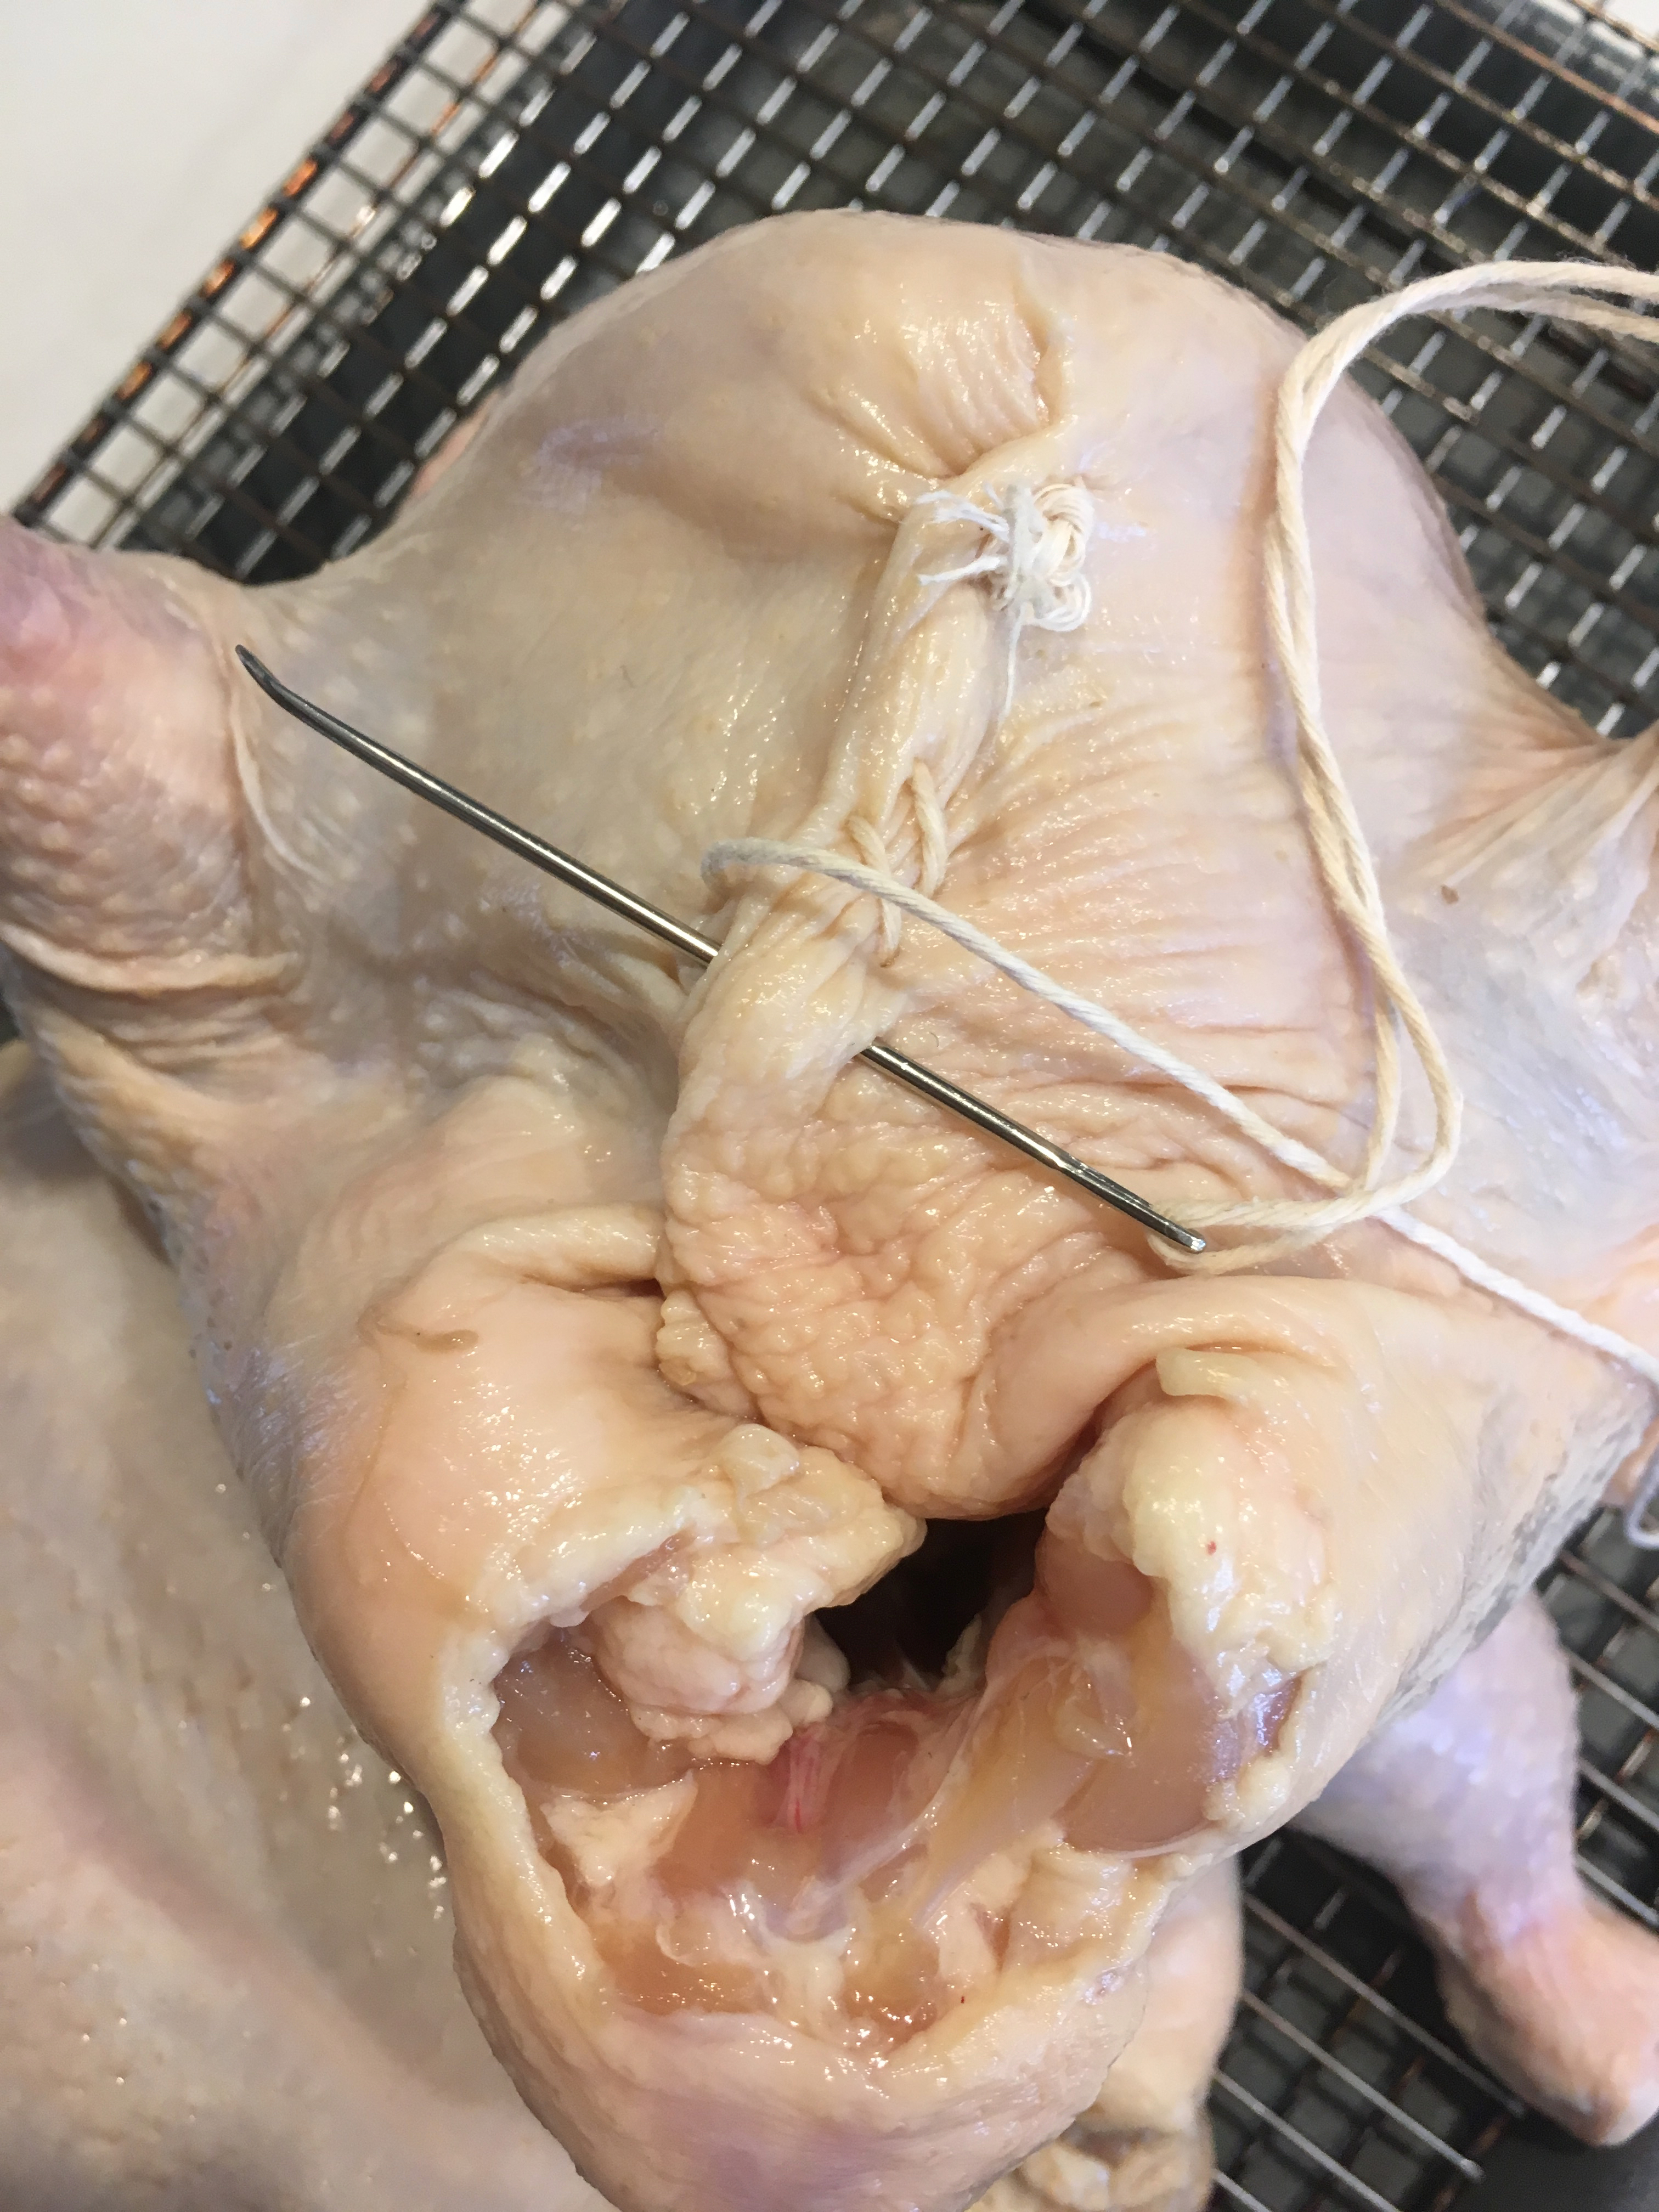
\includegraphics[width=0.25\textwidth]{\imageDir/\fileName/IMG_3214.jpg} &
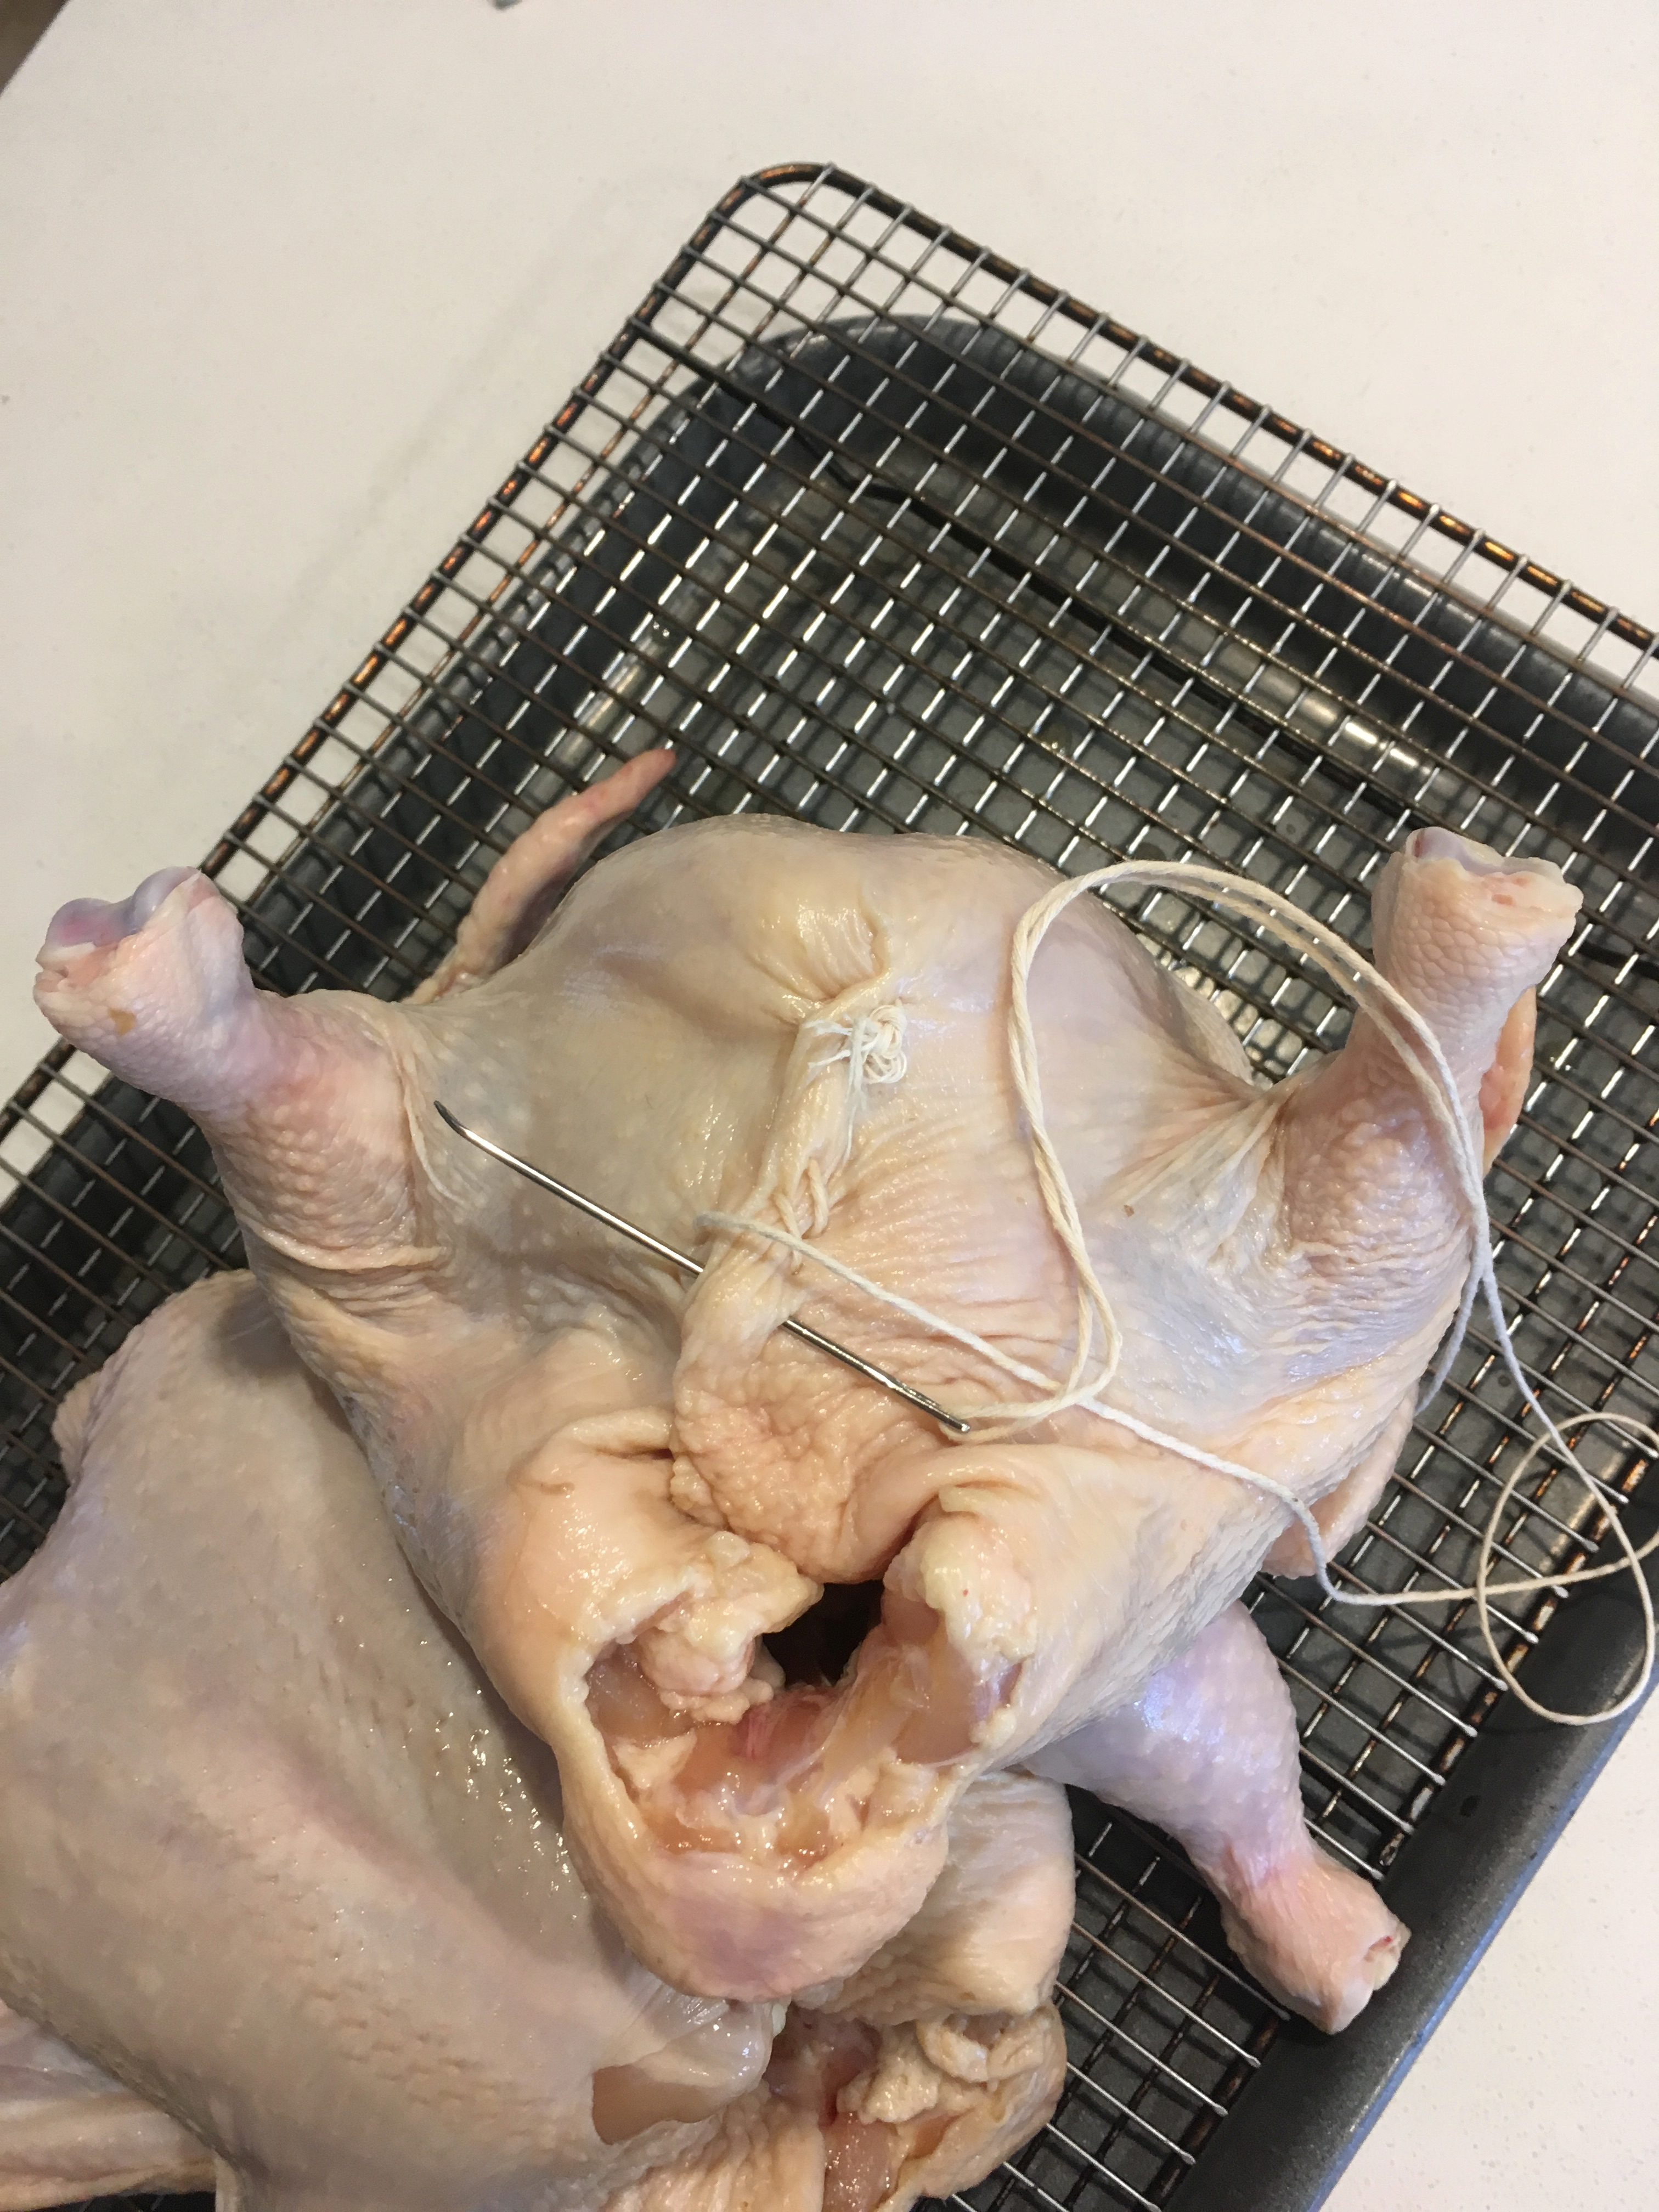
\includegraphics[width=0.25\textwidth]{\imageDir/\fileName/IMG_3216.jpg} \\
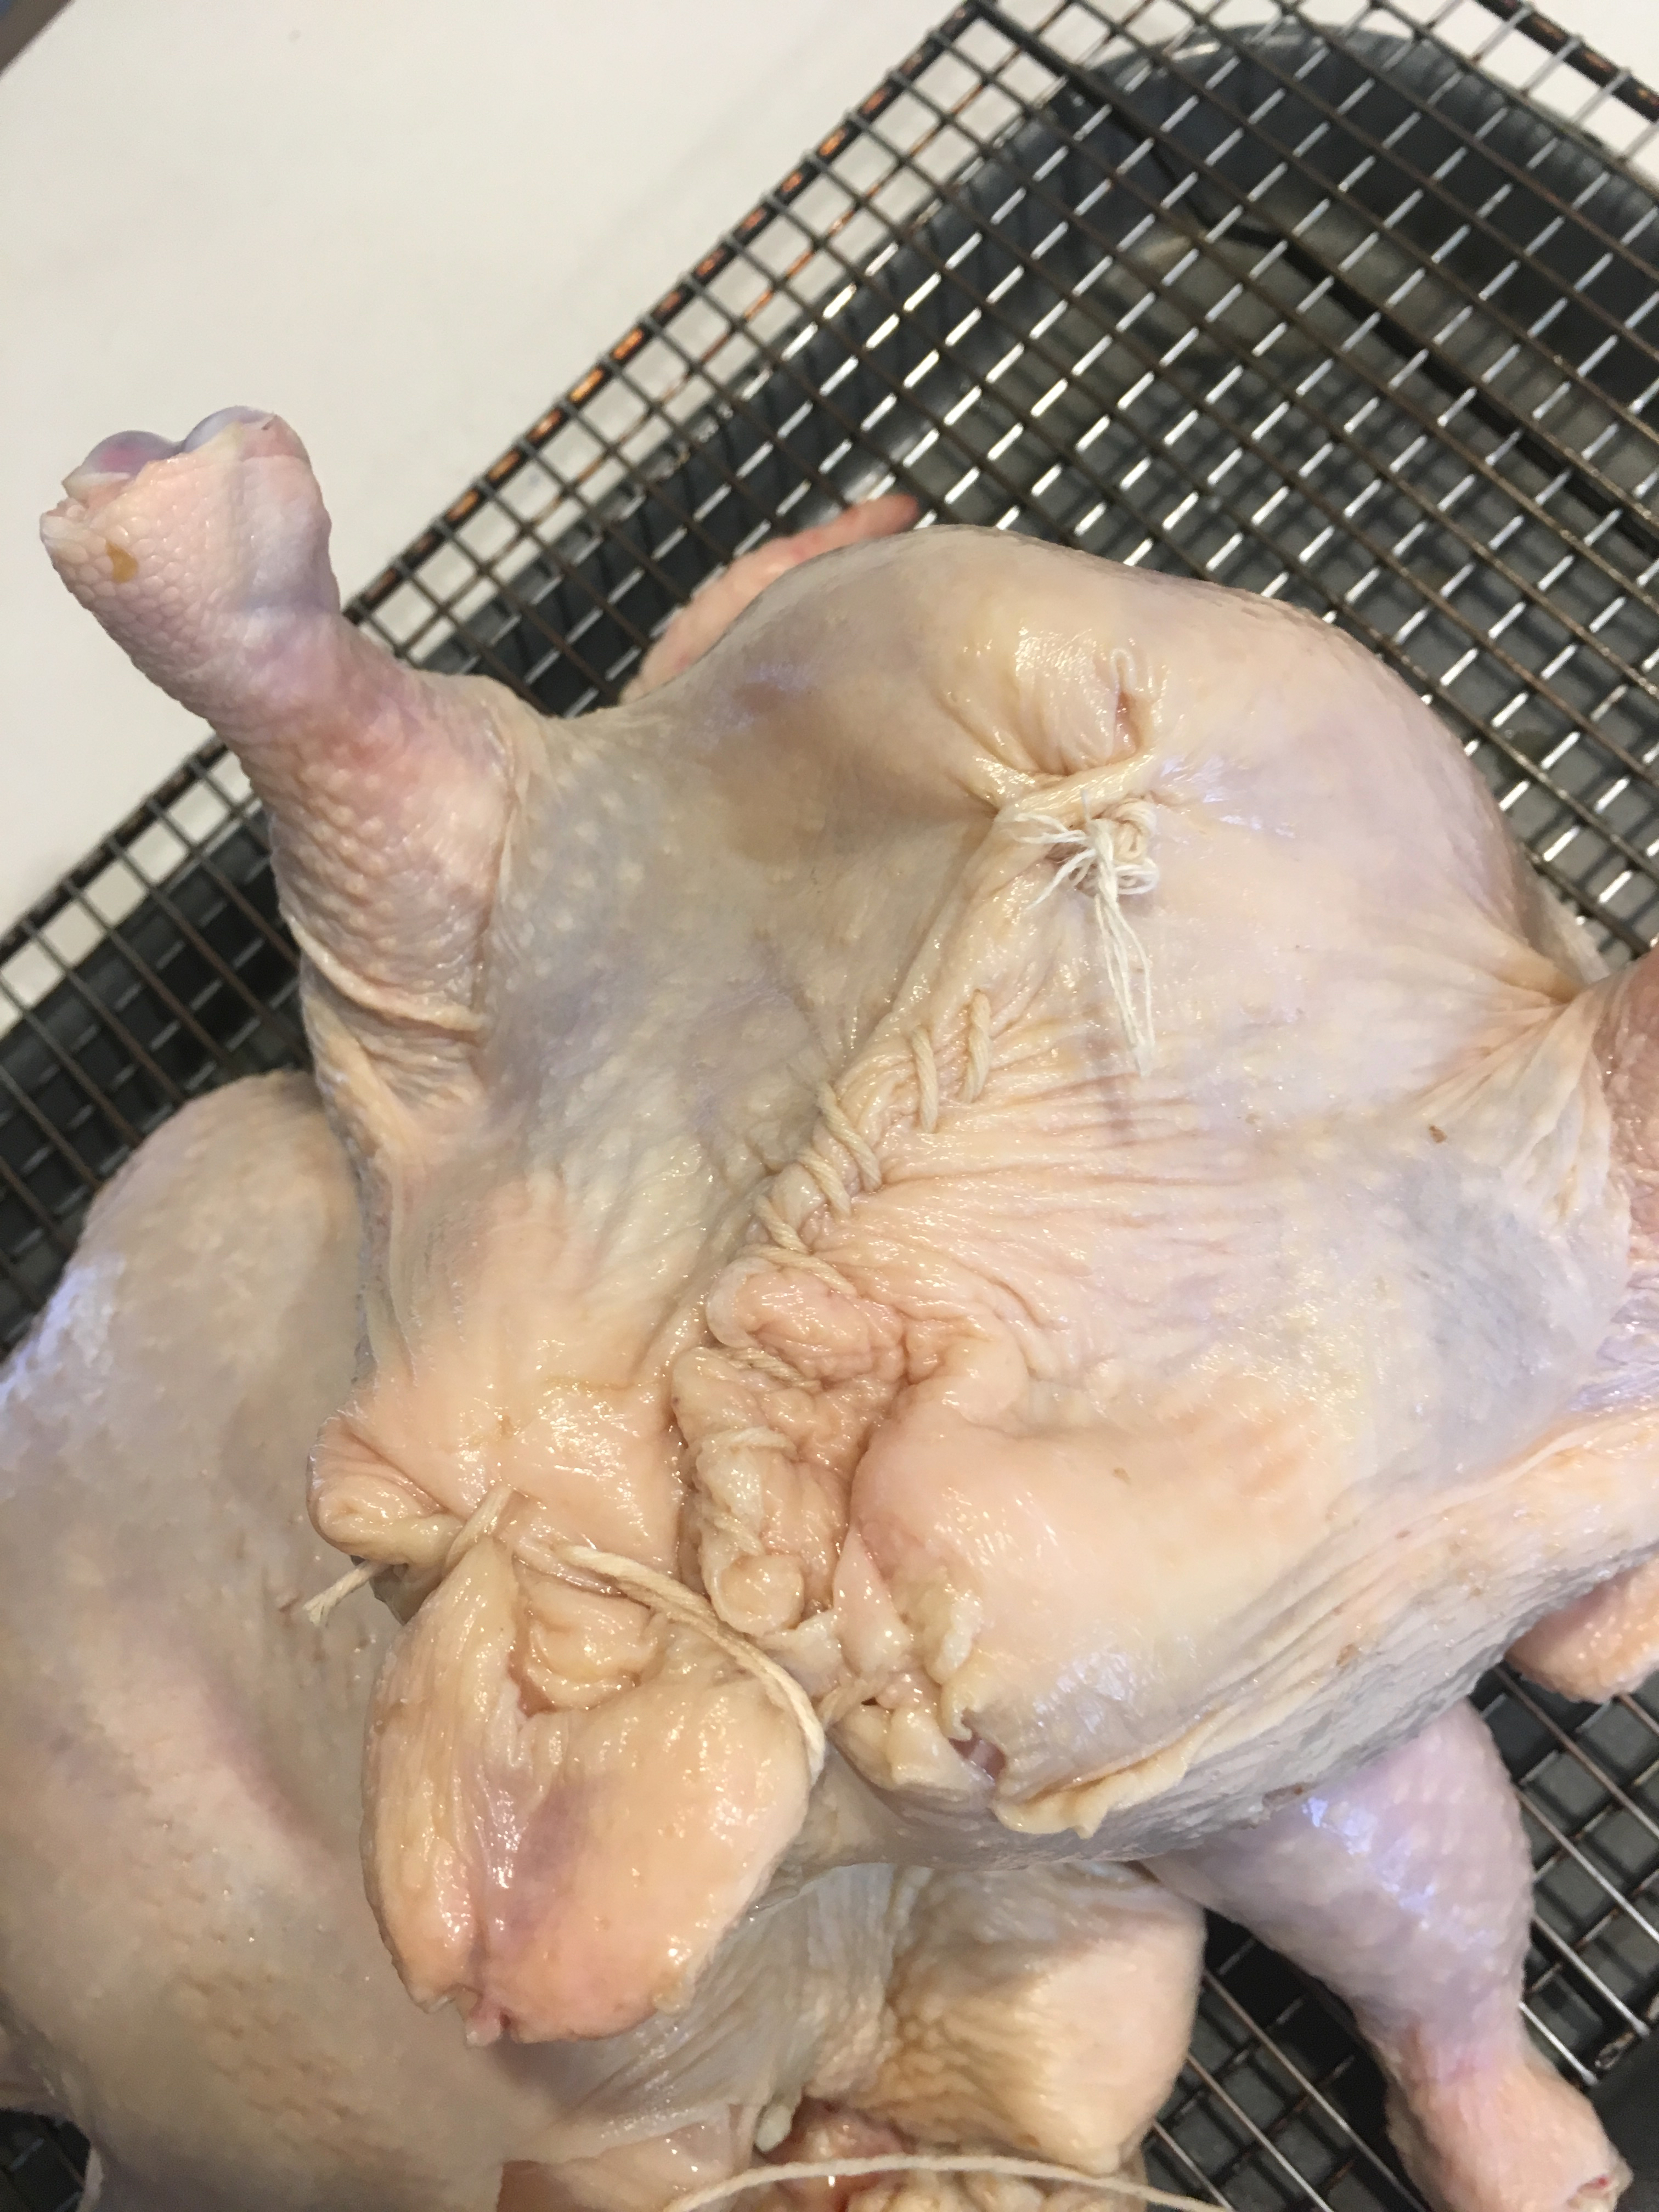
\includegraphics[width=0.25\textwidth]{\imageDir/\fileName/IMG_3217.jpg} &
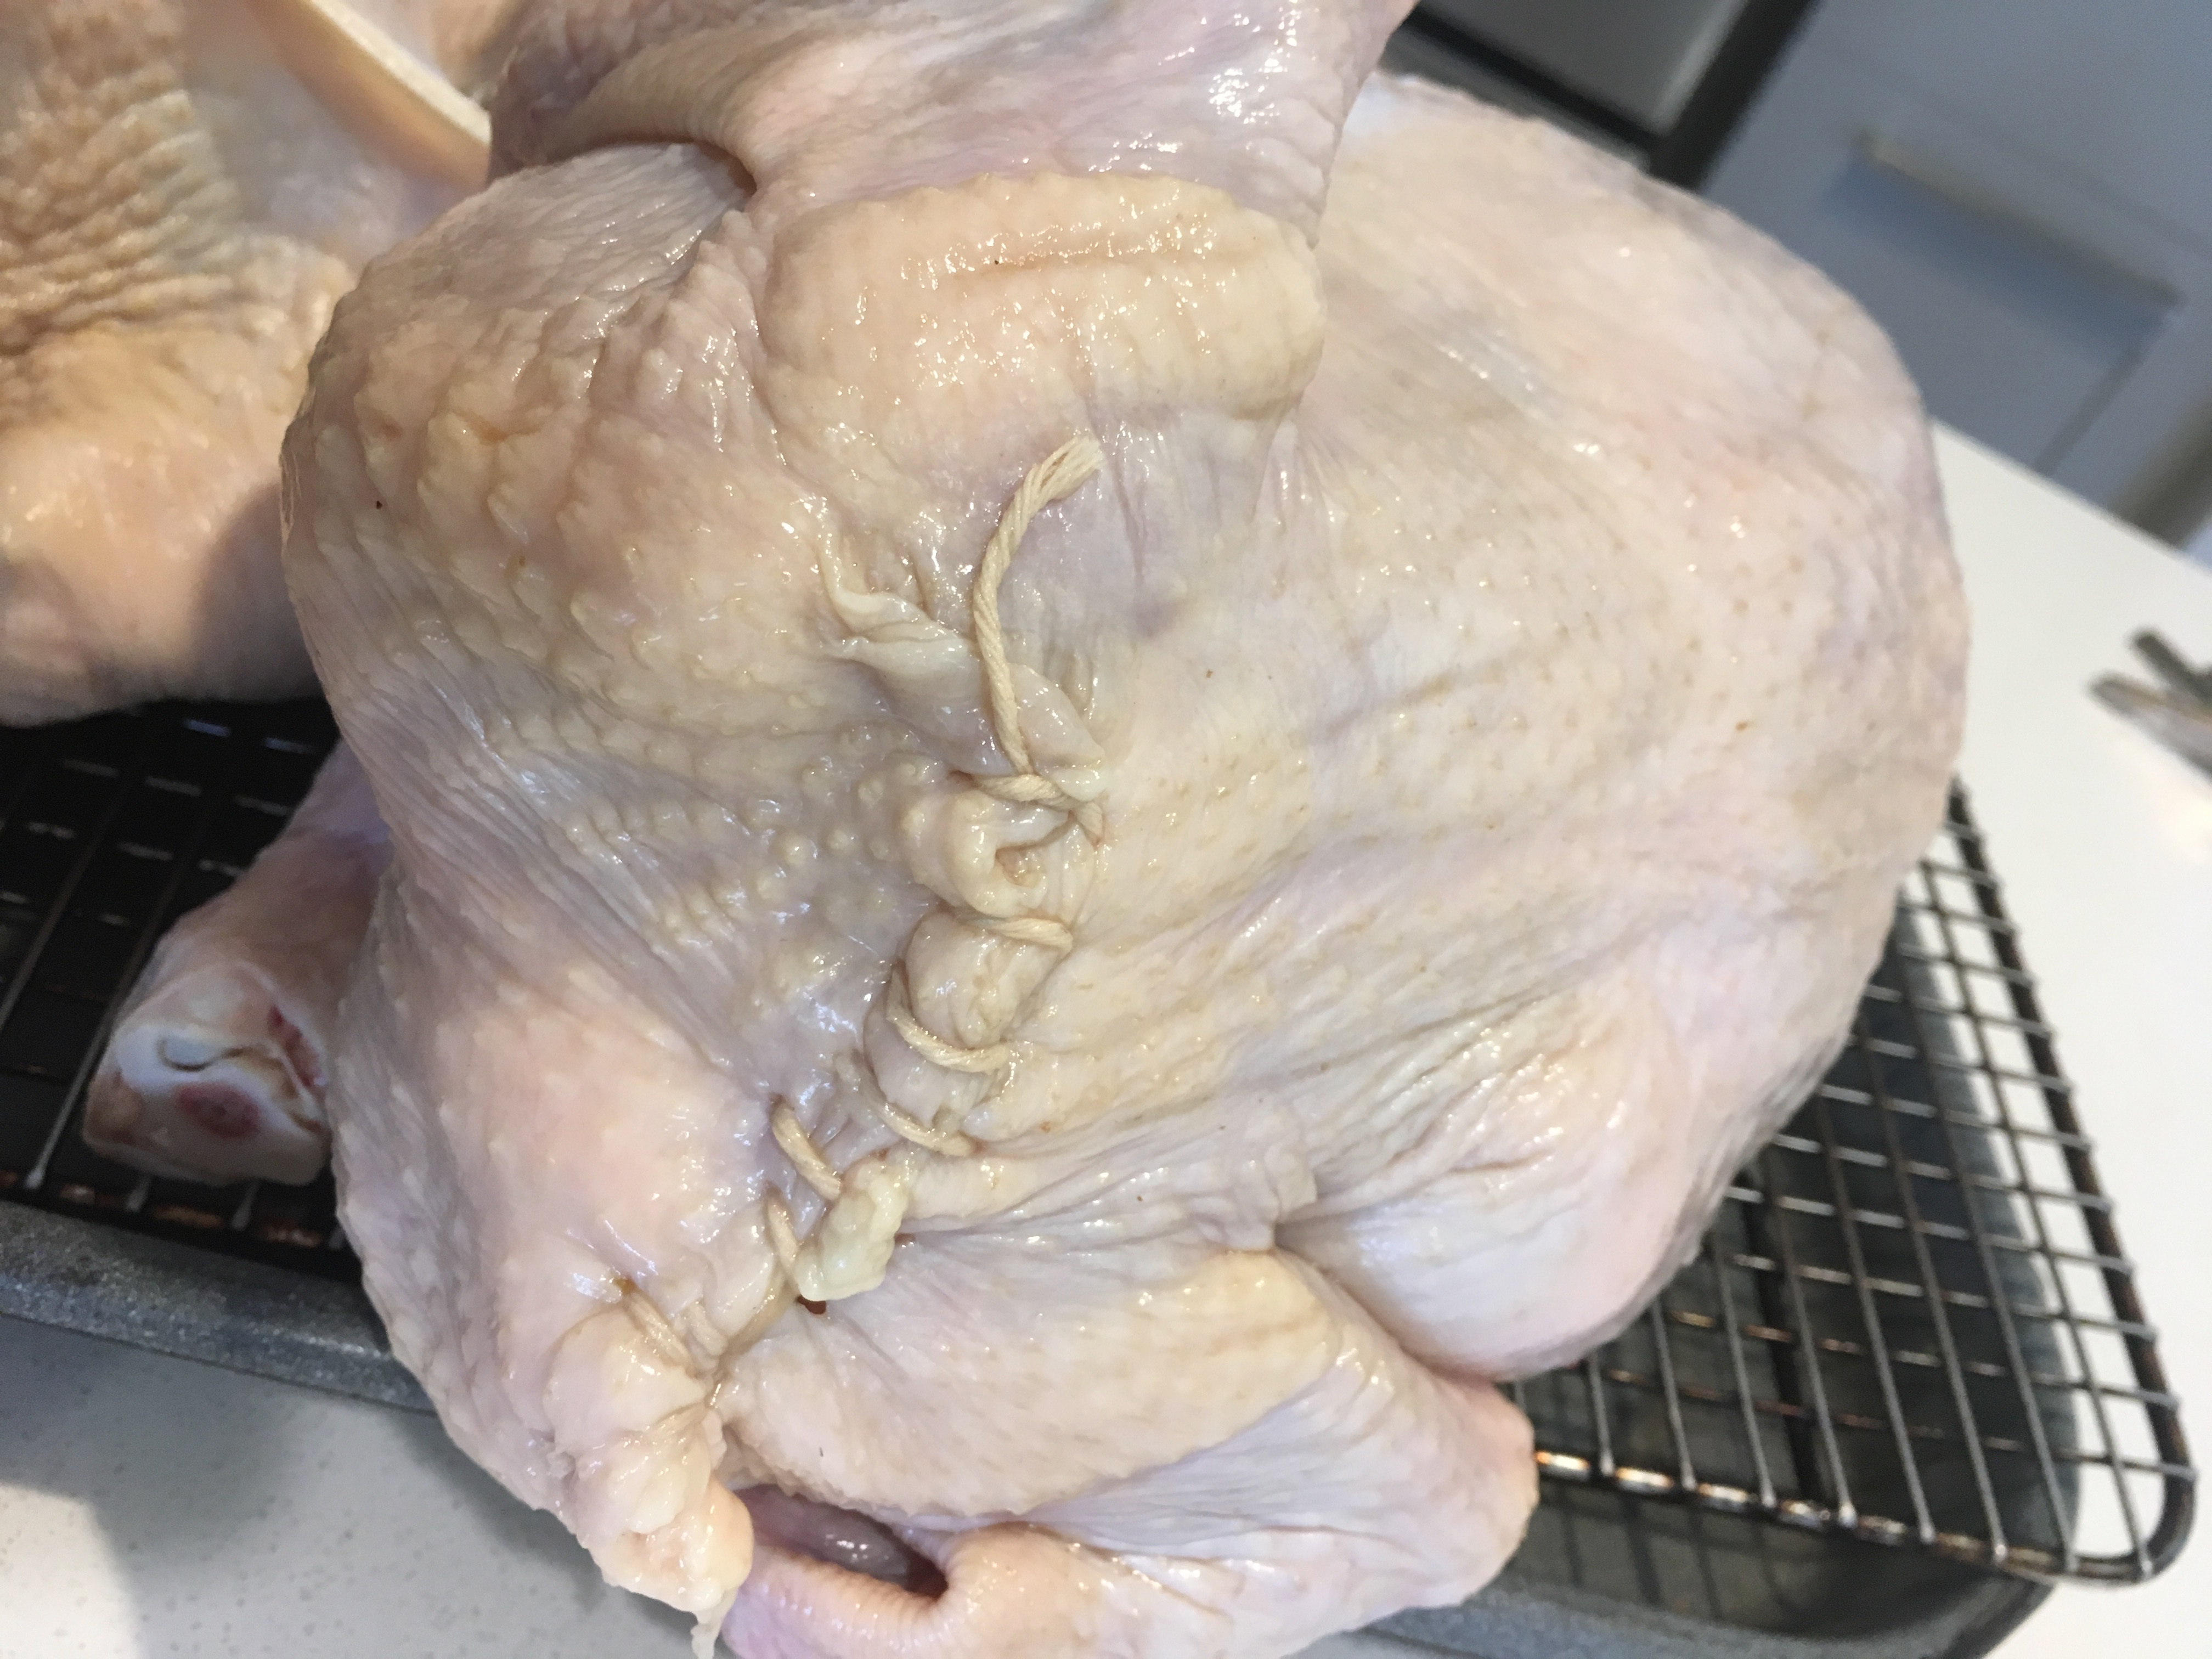
\includegraphics[width=0.25\textwidth]{\imageDir/\fileName/IMG_3218.jpg} &
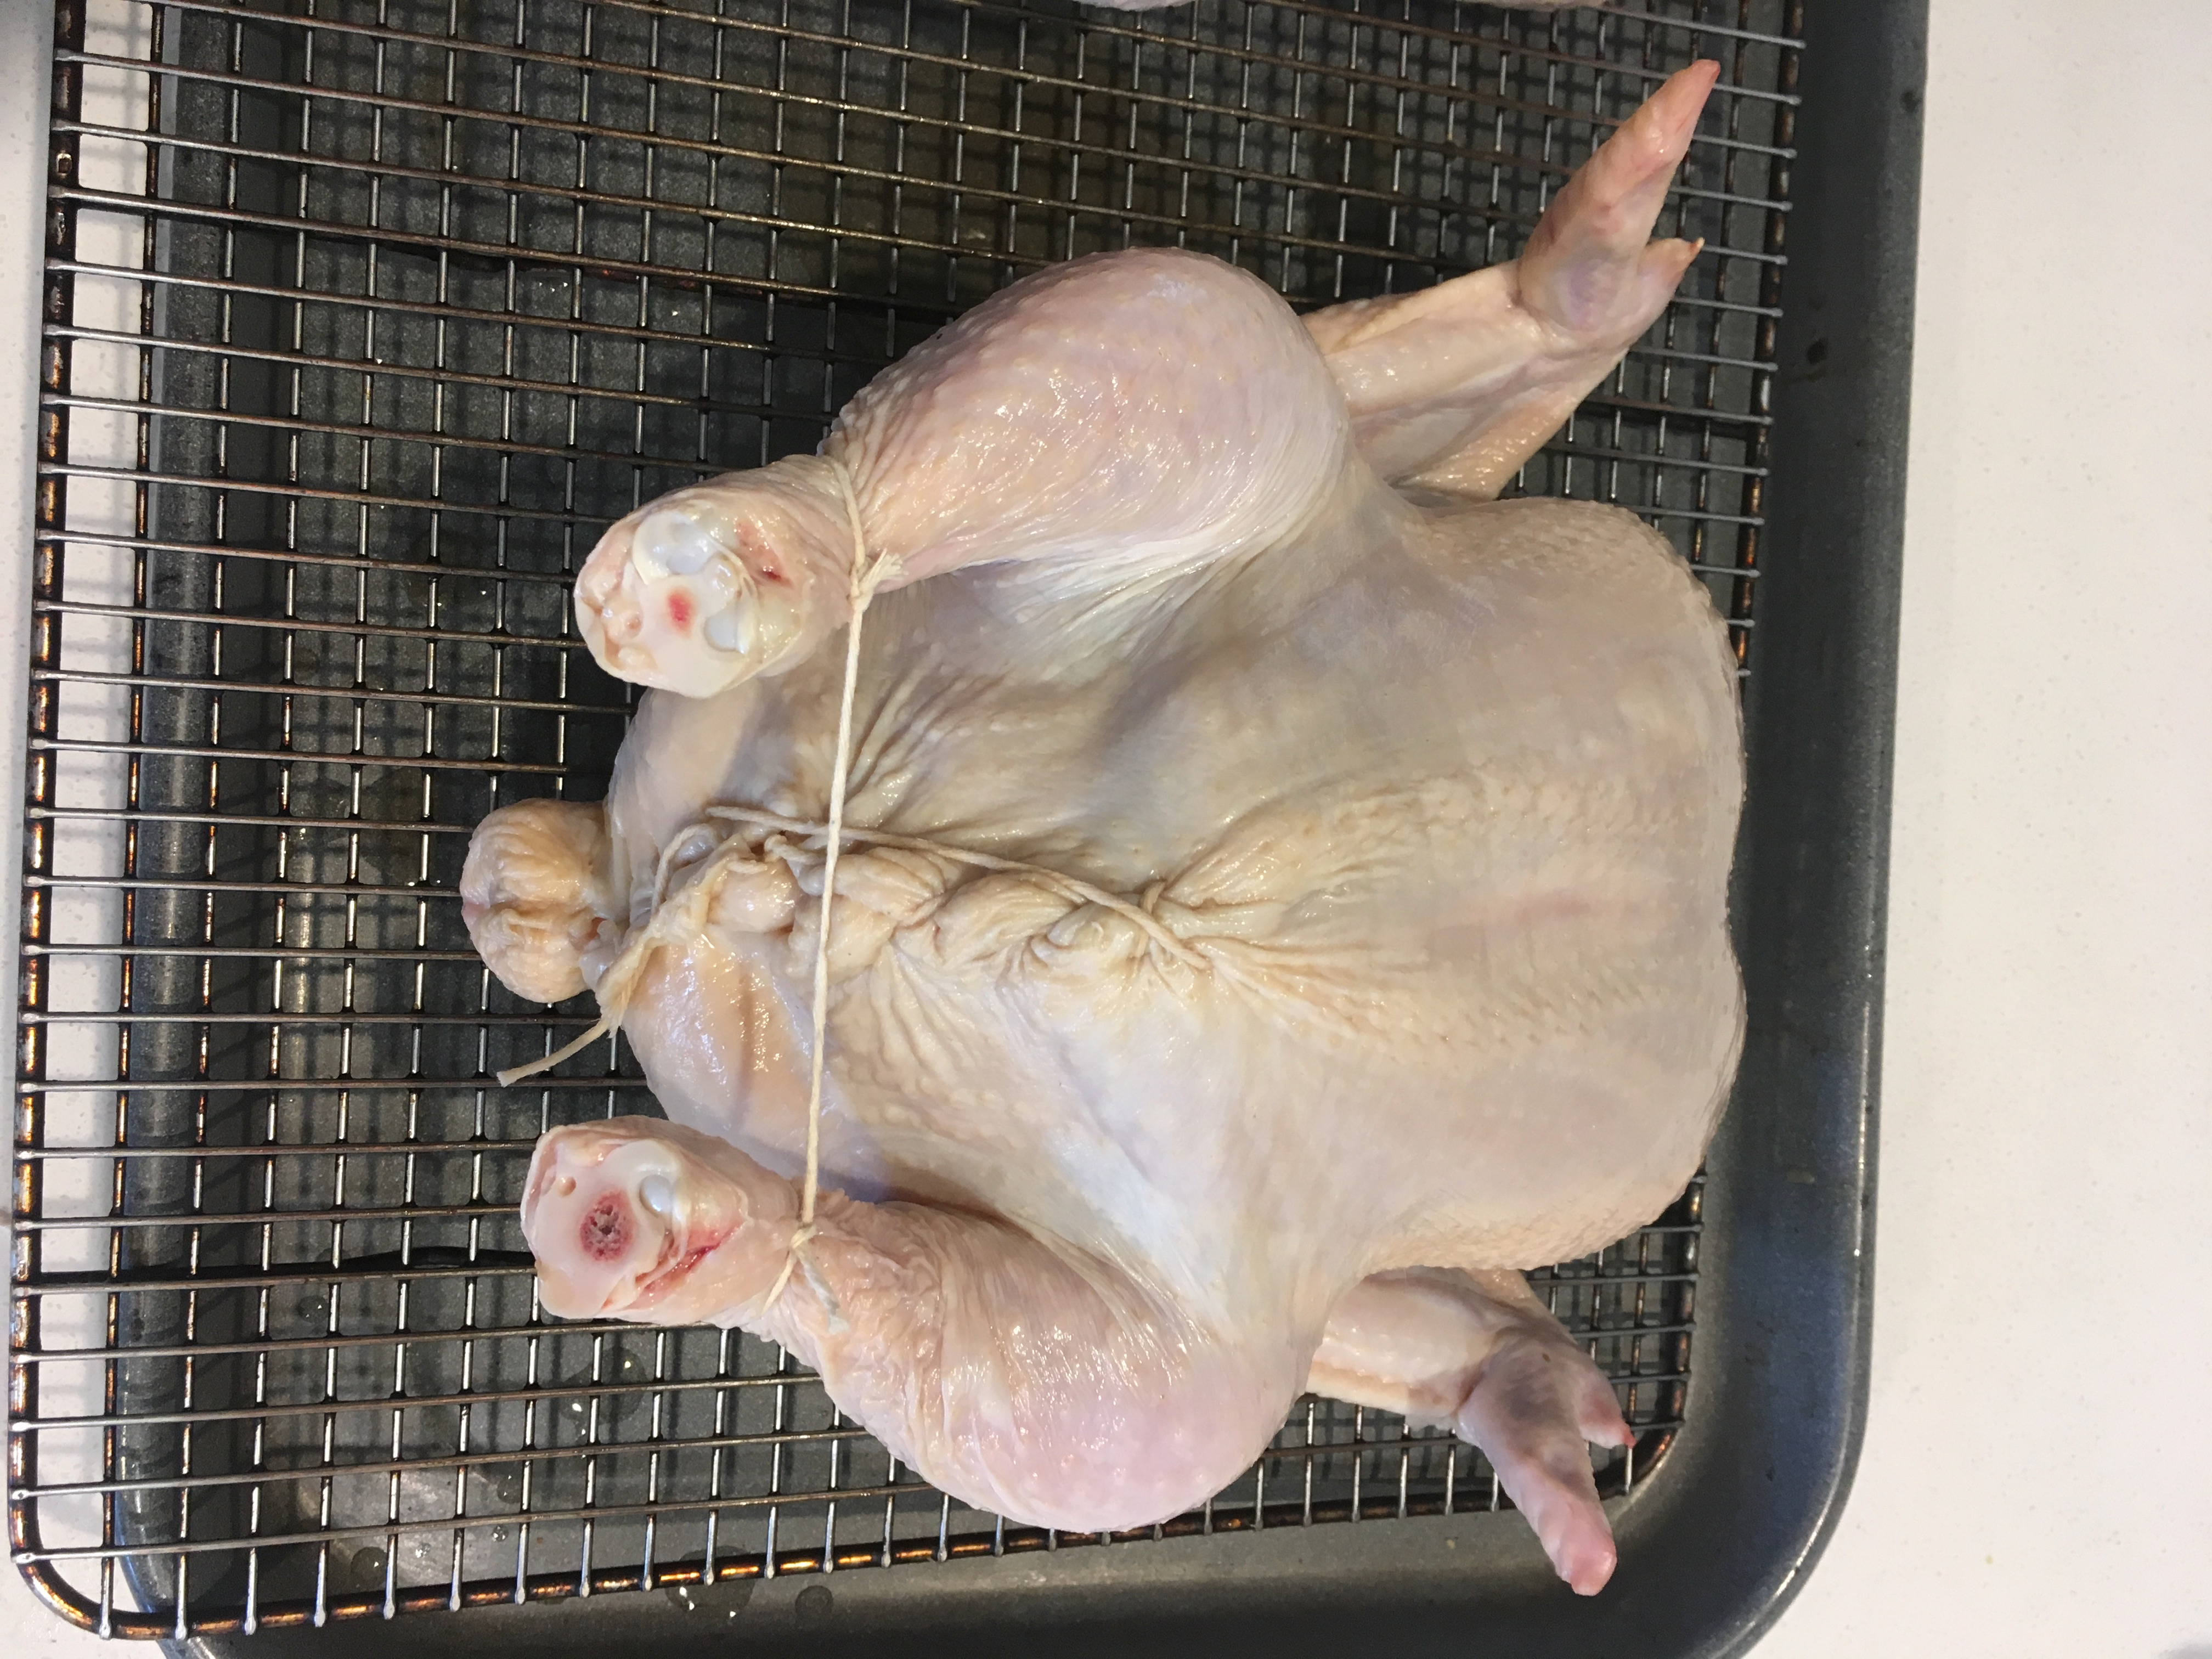
\includegraphics[width=0.25\textwidth]{\imageDir/\fileName/IMG_3219.jpg} \\
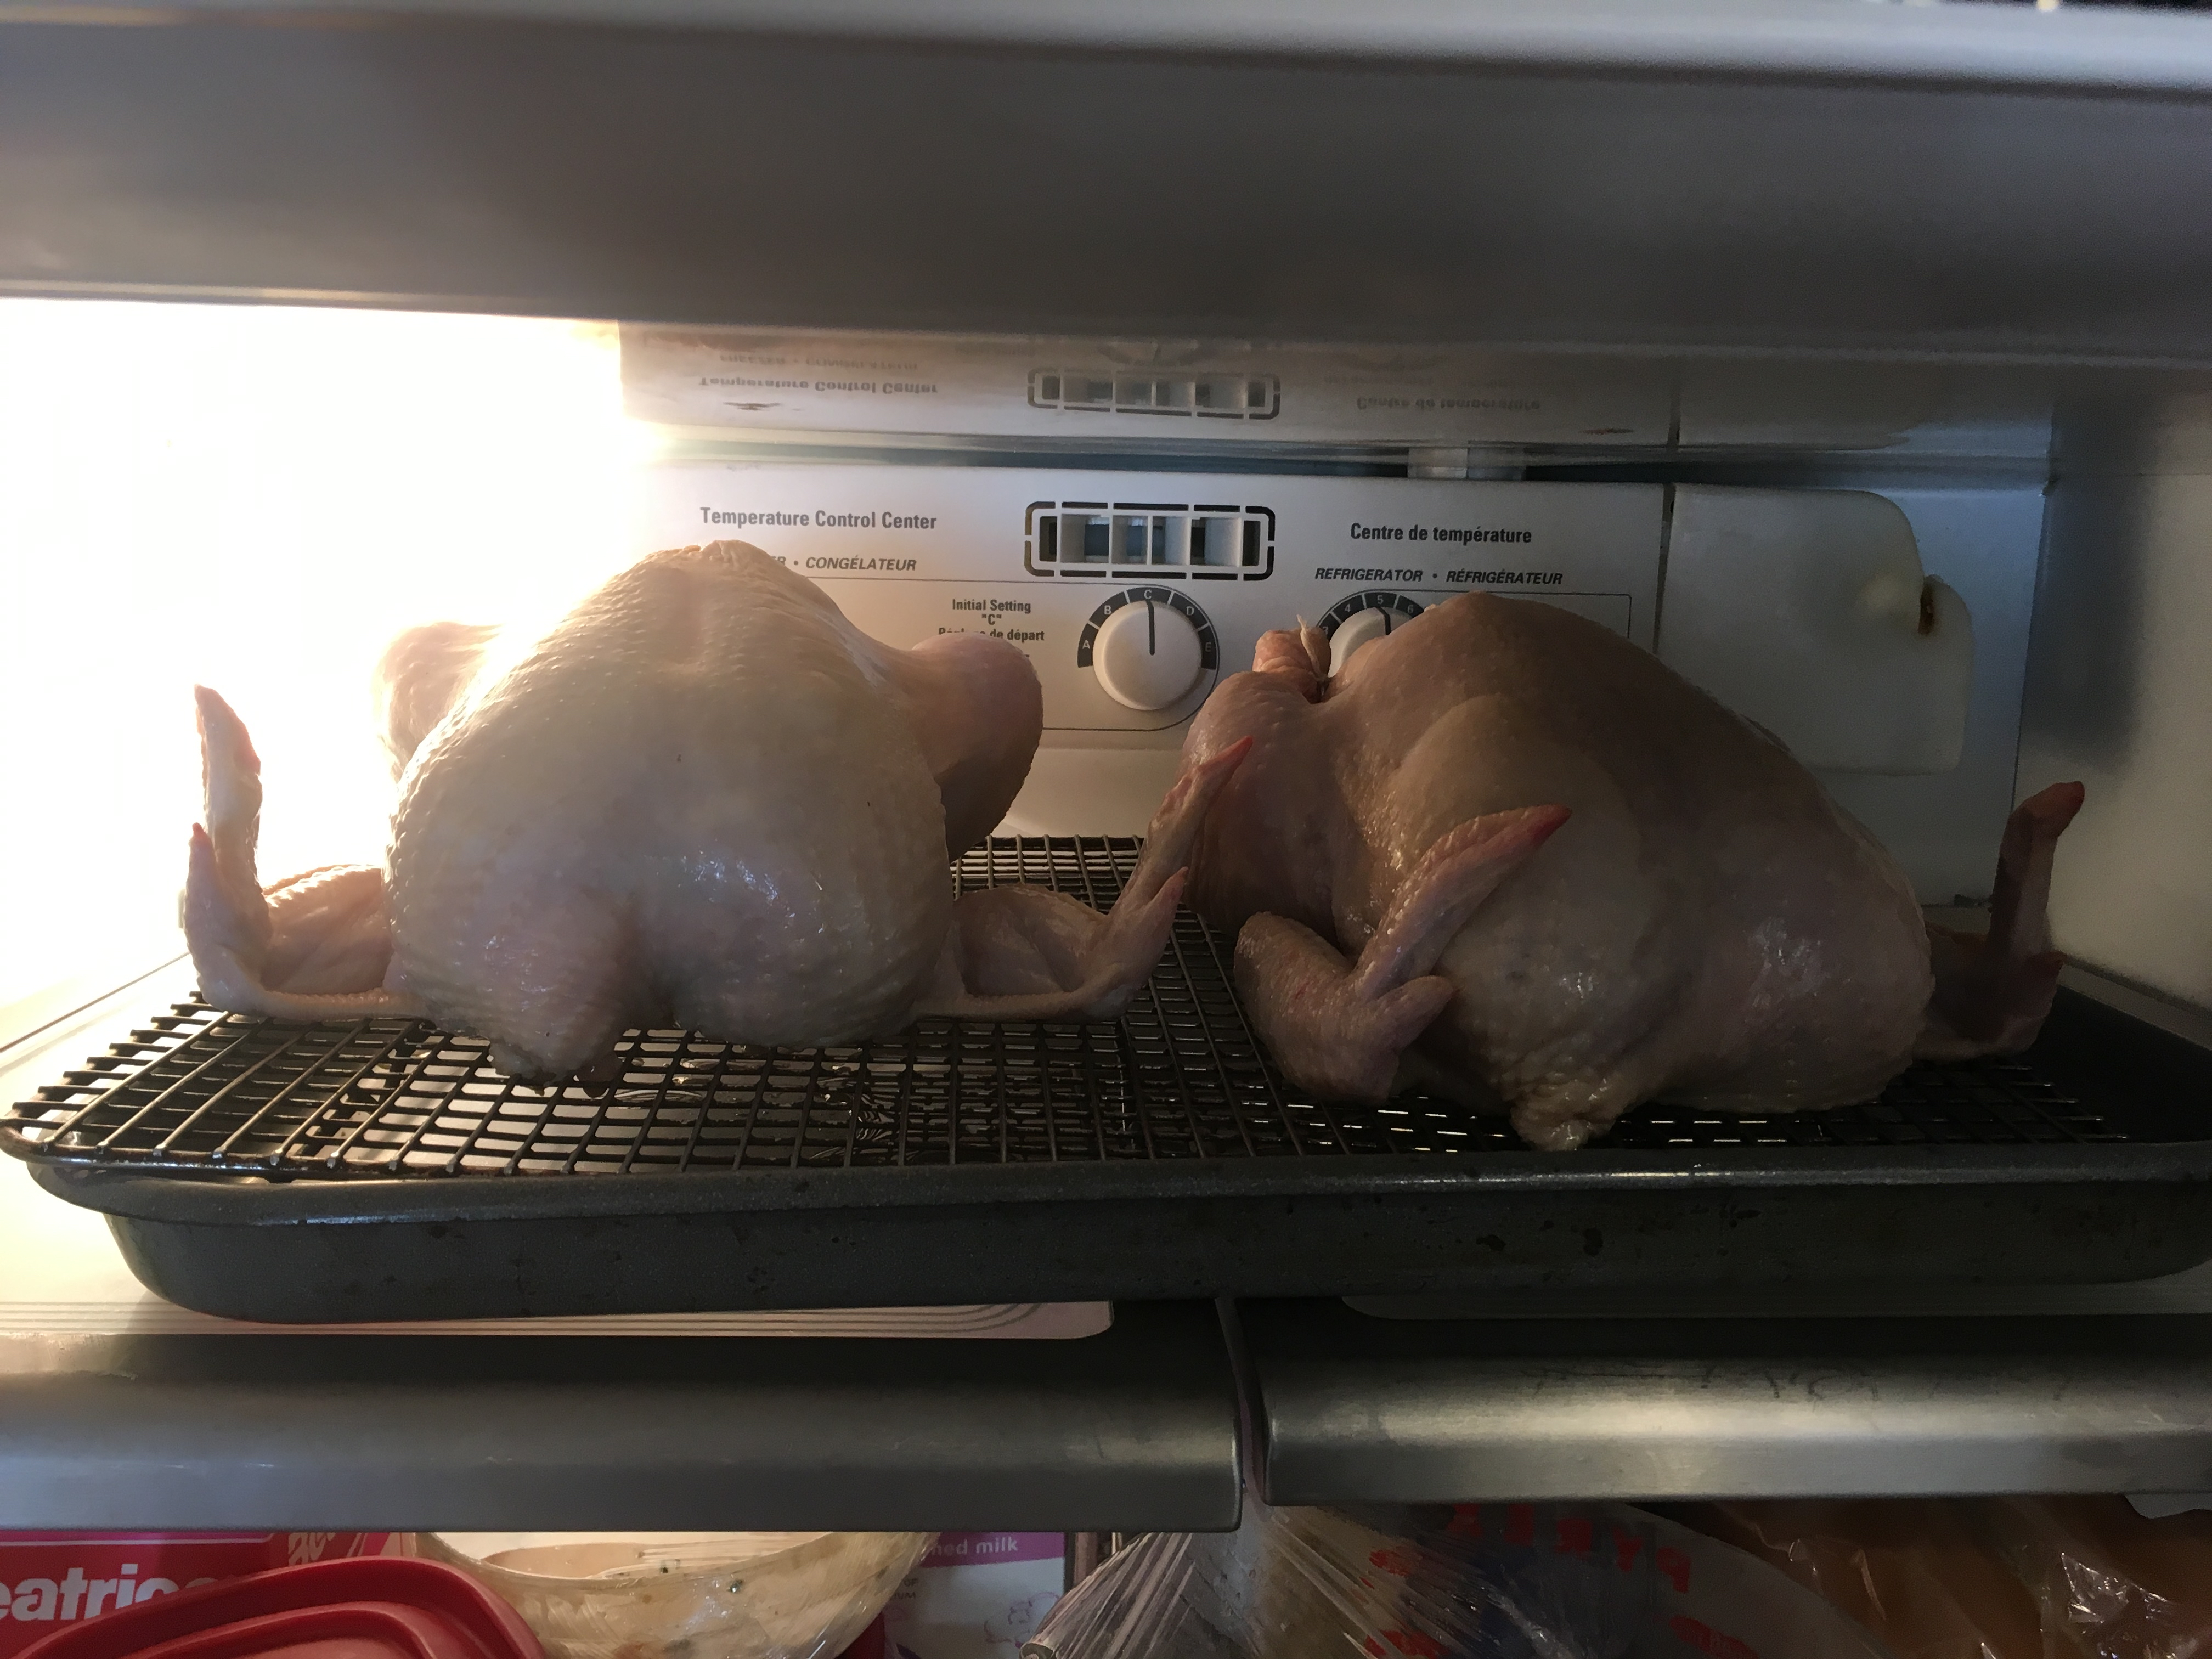
\includegraphics[width=0.25\textwidth]{\imageDir/\fileName/IMG_3220.jpg} &
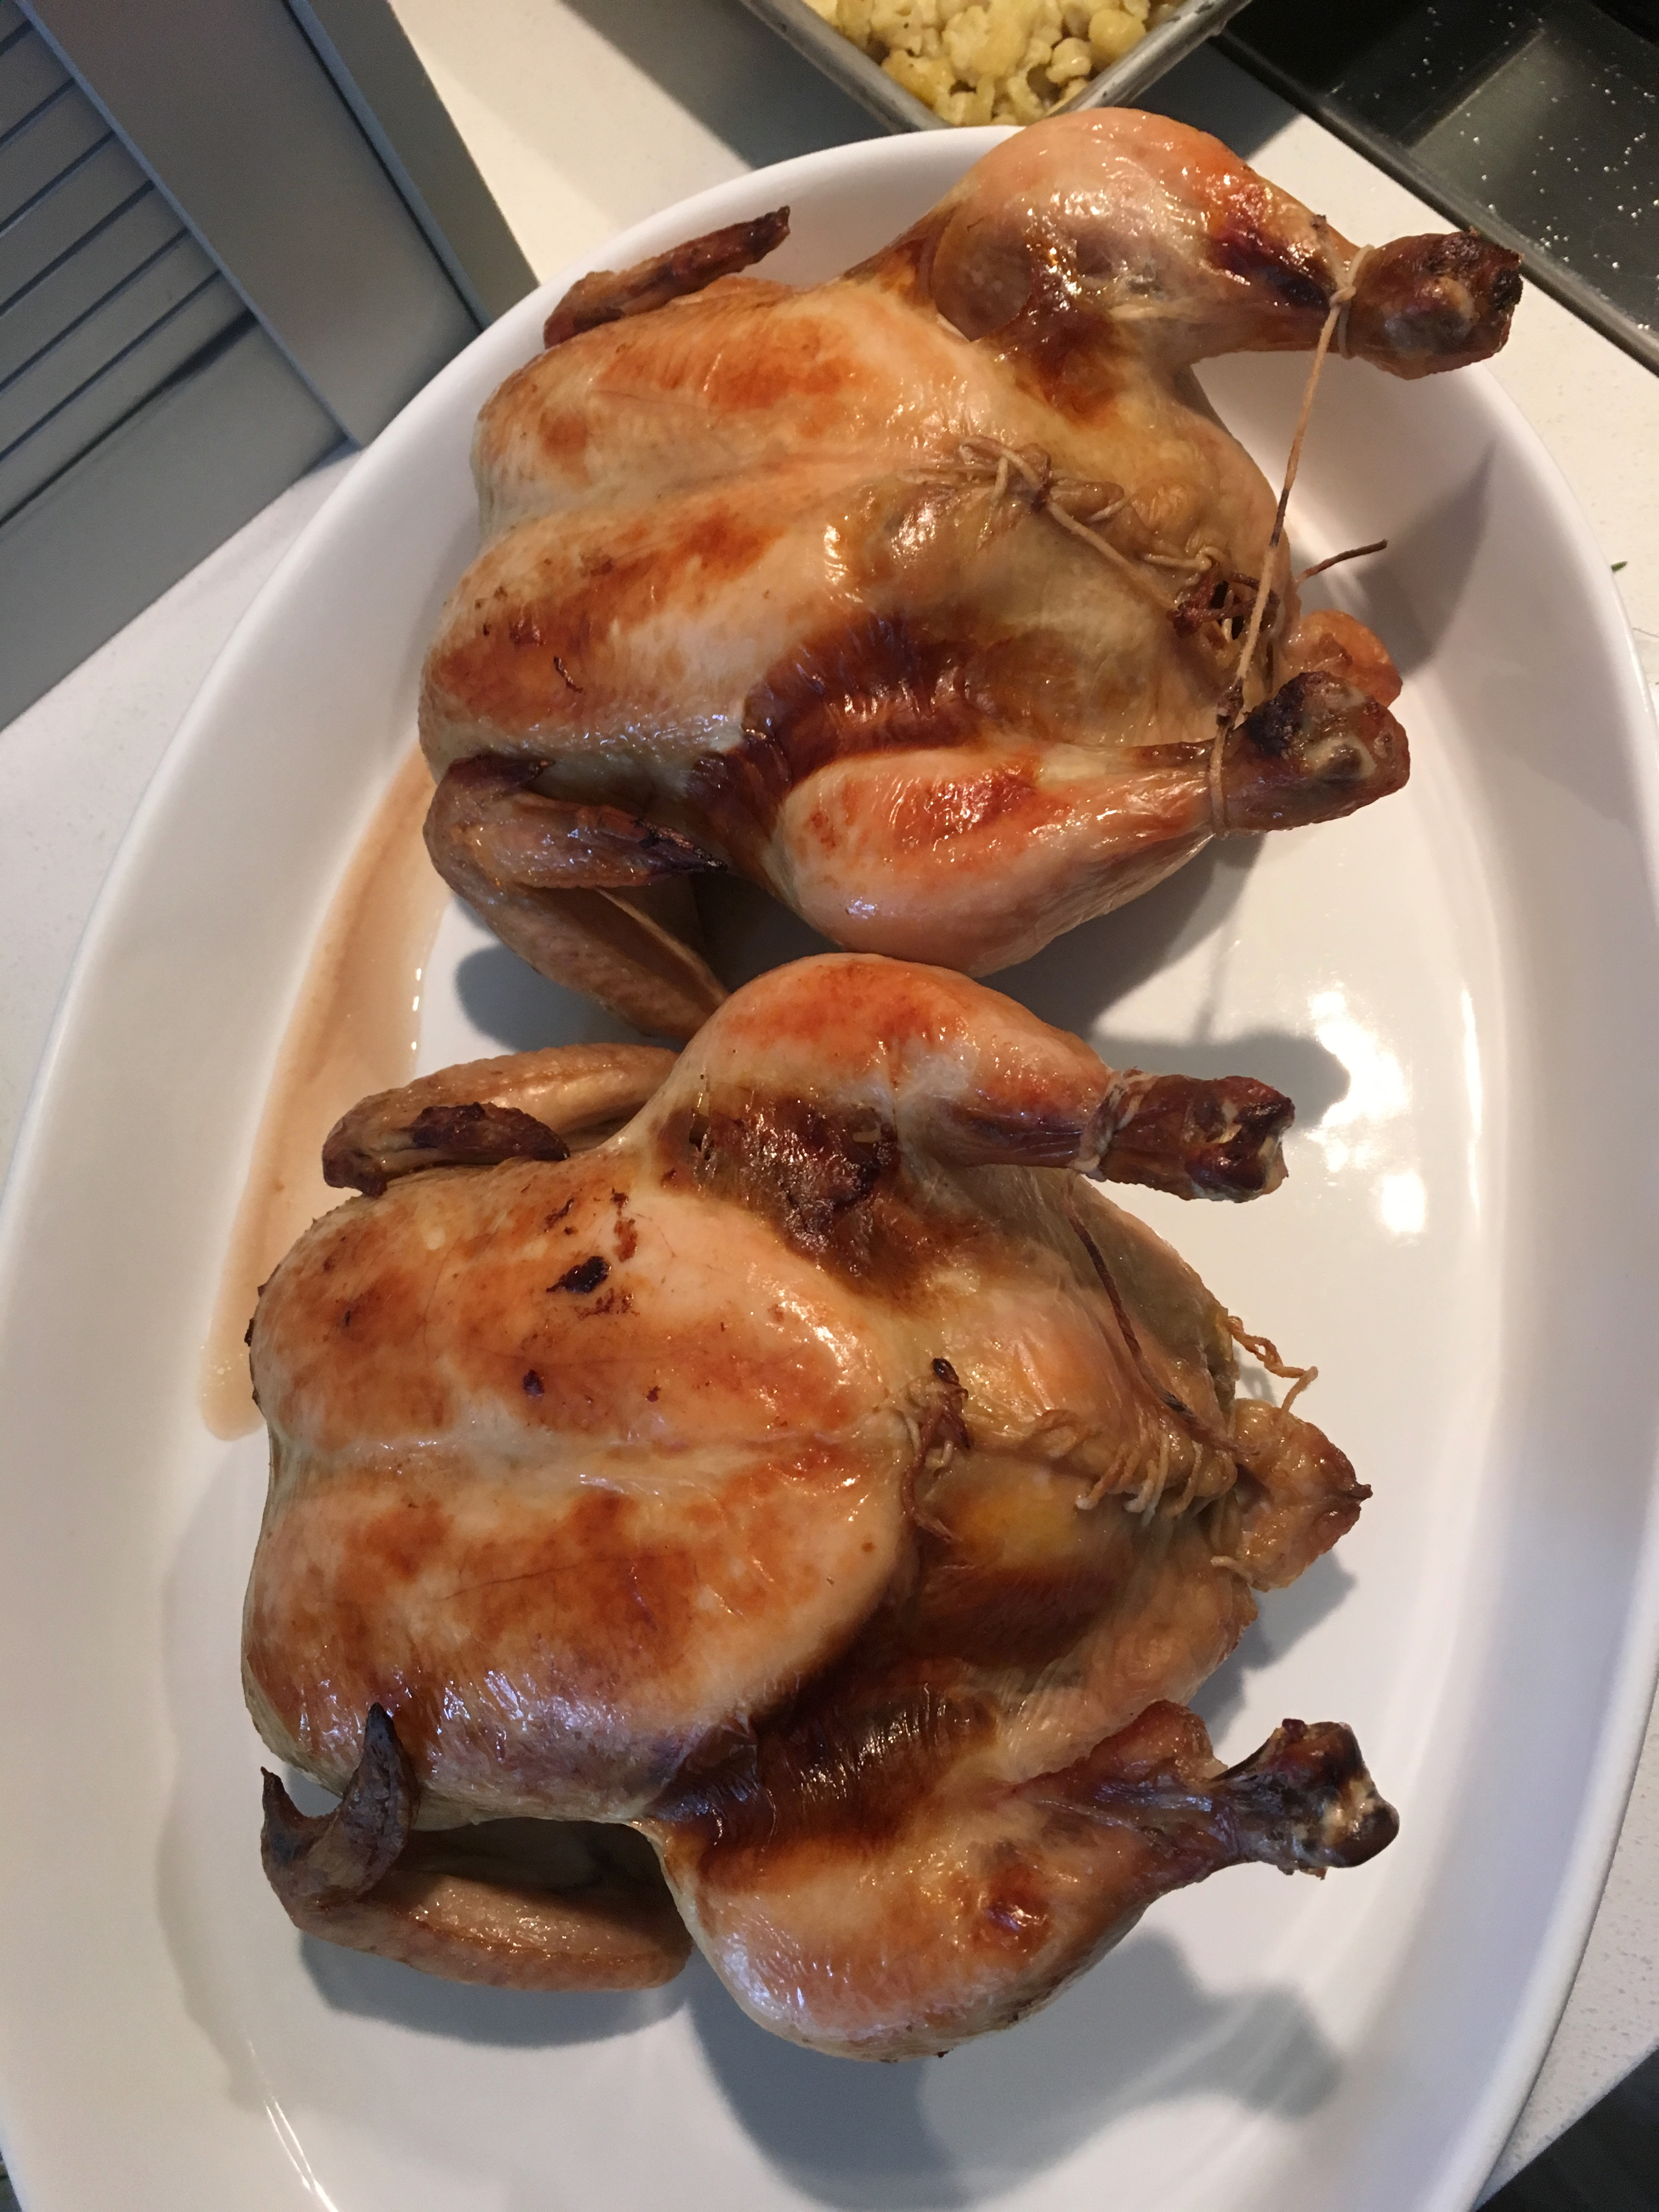
\includegraphics[width=0.25\textwidth]{\imageDir/\fileName/IMG_3228.jpg} \\
\end{tabular}
\end{table}


\end{document}



